\documentclass[12pt]{article}

\usepackage[T2A]{fontenc}
\usepackage[utf8]{inputenc}
\usepackage[english,russian]{babel}

\usepackage{amsmath}
\usepackage{amsthm, mathrsfs, mathtools, amssymb}
\usepackage{enumitem}

\usepackage{epigraph}

\usepackage{tikz}
\usetikzlibrary{decorations.pathmorphing}
% для волнистой линии для фотонов создал стиль линии snake arrow
% рисует волну и на конце ее чуть-чуть прямую линию оставляет для стрелки
\tikzset{snake arrow/.style=
	{->,
		decorate,
		decoration={snake,amplitude=.4mm,segment length=2mm,post length=1mm}},
}
\usepackage{caption}
\usepackage{float}
\usepackage{multirow}
\usepackage{multicol}
\usepackage{wrapfig}
%\usepackage{hyperref}
%\hypersetup{
	%	colorlinks,
	%	citecolor=black,
	%	filecolor=black,
	%	linkcolor=black,
	%	urlcolor=black
	%}

\usepackage{geometry}
\geometry{verbose,a4paper,tmargin=1cm,bmargin=2cm,lmargin=1.5cm,rmargin=1.5cm}

\begin{document}
	%  \tableofcontents \newpage
	
	\section{Теоретическая часть}
	
	\subsection{Линейные уравнения с частными производными первого порядка. Уравнения характеристик. Первый интеграл. Квазилинейные уравнения. Задача Коши.}
\label{firstorder_lineq} \newpage
	\subsection{Классификация линейных уравнений с частными производными 2-го порядка. Характеристическое уравнение. Приведение уравнения с частными производными к каноническому виду.}
\label{sec:types}

Уравнением с частными производными 2-го порядка с двумя независимыми переменными $x, y$ называетс соотношение между неизвестной функцией $ u(x, y)$ и ее частными производными до 2-го порядка включительно:\footnote{Т.-С. стр. 15 и далее}
\begin{equation}
	F(x, y, u, u_x, u_y, u_{xx}, u_{xy}, u_{yy}) = 0.
\end{equation}

Уравнение называется линейным относительно старших производных, если оно имеет вид
\begin{equation} \label{SOlineq}
	a_{11} u_{xx} + 2 a_{12} u_{xy} + a_{22} y_{yy} + F_1(x, y, u, u_x, u_y) = 0,
\end{equation}
где $a_{11}, a_{12}, a_{22}$ являются функциями $x$ и $y$.

Уравнение называется линейным, если оно линейно как относительно старших производных $u_{xx}, u_{xy}, u_{yy}$, так и относительно функции $u$ и ее первых производных $u_x, u_y$:
\begin{equation} \label{SOeq}
	a_{11}  u_{xx} + 2 a_{12} u_{xy} + a_{22} + b_1 u_x + b_2 u_y + c u + f = 0. 
\end{equation}
где $a_{11}, a_{12}, a_{22}, b_1, b_2, c, f$ --- функции от $x$ и $y$. Уравнение называется однородным, если $f(x, y) = 0$.

Аналогично линейным уравнениям с частными производными 1-го порядка, линейные уравнения с частными производными 2-го порядка называются \textit{квазилинейными}, если коэффициенты $a_{11}, a_{12}, a_{22}$ подобно $F_1$ зависят от $x, y, y, u_x, u_y$. 

С помощью преобразования переменных
\begin{equation*}
	\xi = \varphi(x, y), \quad \eta = \psi(x, y),
\end{equation*}
допускающего обратное преобразование, мы получаем новое уравнение, эквиввалентное исходному. Как выбрать $\xi$ и $\eta$ так, тчобы получить наиболее простой вид?

Получим ответ на поставленный вопрос для \eqref{SOlineq}. Преобразуя производные к новым переменным, получаем
\begin{equation} \label{varchange}
	\begin{rcases}
		u_x = u_{\xi} \xi_{x} + u_{\eta} \eta_{x}, \\
		u_y = u_{\xi} \xi_{y} + u_{\eta} \eta_{y}, \\
		u_{xx} = u_{\xi\xi} \xi_{x}^2 + 2 u_{\xi\eta} \xi_{x} \eta_{x} + u_{\eta\eta} \eta^2_{x} + u_{\xi} \xi_{xx} + u_{\eta} \eta_{xx}, \\
		u_{xy} = u_{\xi\xi} \xi_{x} \xi_{y} + u_{\xi\eta}(\xi_x \eta_y + \xi_y \eta_x) + u_{\eta\eta} \eta_x \eta_y + u_{\xi} \xi_{xy} + u_{\eta} \eta_{xy}, \\
		u_{yy} = u_{\xi\xi} \xi_{y}^2 + 2 u_{\xi\eta} \xi_{y} \eta_{y} + u_{\eta\eta} \eta^2_{y} + u_{\xi} \xi_{yy} + u_{\eta} \eta_{yy},
	\end{rcases}
\end{equation}
Подставляя значения производных из \eqref{varchange} в уравнение \eqref{SOlineq}, будем иметь 
\begin{equation} \label{SOeqCHANGED}
	\bar{a}_{11} u_{\xi\xi} + 2 \bar{a}_{12} u_{\xi\eta} + \bar{a}_{22} u_{\eta\eta} + \bar{F} = 0,
\end{equation}
где 
\begin{align*}
	&\bar{a}_{11} = a_{11} \xi^2_{x} + 2 a_{12} \xi_x \xi_y + a_{22} \xi^2_y, \\
	&\bar{a}_{12} = a_{11} \xi_x \eta_x + a_{12} (\xi_x \eta_y + \eta_x \xi_y) + a_{22} \xi_{y} \eta_{y}, \\
	&\bar{a}_{22} = a_{11} \eta^2_{x} + 2 a_{12} \eta_x \eta_y + a_{22} \eta^2_y,
\end{align*}
а функция $\bar{F}$ не зависит от вторых производных. Заметим, что если исходное уравнение линейно, т.е. 
\begin{equation*}
	F(x, y, u, u_x, u_y) = b_1 u_x + b_2 u_y + c u + f,
\end{equation*}
то $\bar{F}$ имеет вид 
\begin{equation*}
	\bar{F}(\xi, \eta, u, u_{\xi}, u_{\eta}) = \beta_1 u_{\xi} + \beta_2 u_{\eta} + \gamma u + \delta,
\end{equation*}
т.е. уравнение остается линейным. 

Выберем переменные $\xi$ и $\eta$ так, чтобы коэффициент $\bar{a}_{11}$ был равен нулю. Рассмотрим уравнение с частными производными 1-го порядка
\begin{equation} \label{FOeq}
	a_11 z^2_x + 2 a_{12} z_x z_y + a_{22} z_y^2 = 0.
\end{equation}
Пусть $z = \varphi(x, y)$ --- какое-нибудь частное решение этого уравнения. Если положить $\xi = \varphi(x, y)$, то коэффициент $\bar{a}_{11}$, очевидно, будет равен нулю Таким образом, упомянутая выше задача о выборе новых независимых переменных связана с решением уравнения \eqref{FOeq}.  

Если $z = \varphi(x, y)$ является частным решением уравнения \eqref{FOeq}, то соотношение $\varphi(x, y) = C$ представляет собой общий интеграл обыкновенного дифференциального уравнения 
\begin{equation} \label{chareq}
	a_{11} dy^2 - 2 a_{12} dx dy + a_{22} dx^2 = 0.
\end{equation}

Если $\varphi(x, y) = C$ представляет собой общий интеграл обыкновенного дифференциального уравнения \eqref{chareq}, то функция $z = \varphi(x, y)$ удовлетворяет уравнению \eqref{FOeq}. 

Уравнение \eqref{chareq} называется \textit{характеристическим} для уравнения \eqref{SOlineq}, а его интегралы - \textit{характеристиками}. 

Пологая $\xi = \varphi(x, y)$, где $\varphi(x, y) = const$ есть общий интеграл уравнения \eqref{chareq}, мы обращаем в нуль коэффициент при $u_{\xi\xi}$. Если $\psi(x, y) = const$ является другим общим интегралом уравнения \eqref{chareq}, независимым от $\varphi(x, y)$, то, пологая $\eta = \psi(x, y)$, мы обратим в нуль также и коэффициент при $u_{\eta\eta}$. 

Уравнение \eqref{chareq} распадается на два уравнения:
\begin{align}
	\frac{dy}{dx} = \frac{a_{12} + \sqrt{a_{12}^2 - a_{11} a_{22}}}{a_{11}}, \\
	\frac{dy}{dx} = \frac{a_{12} - \sqrt{a_{12}^2 - a_{11} a_{22}}}{a_{11}}.
\end{align}

Знак подкоренного выражения определяет тип уравнения \eqref{SOlineq}
\begin{equation*}
	a_{11} u_{xx} + 2 a_{12} u_{xy} + a_{22} u_{yy} + F = 0.
\end{equation*}

Это уравнение мы будем называть в точке $M$ уравнением:
\begin{align*}
	&\texttt{гиперболического } \text{типа, если в точке } M \, \, a_{12}^2 - a_{11} a_{22} > 0, \\
	&\texttt{параболического } \text{типа, если в точке } M \,\, a_{12}^2 - a_{11} a_{22} = 0, \\
	&\texttt{эллиптического } \text{типа, если в точке } M \,\, a_{12}^2 - a_{11} a_{22} < 0.
\end{align*}
Нетрудно убедиться в правильности соотношения
\begin{equation*}
	\bar{a}_{12}^{2} - \bar{a}_{11} \bar{a}_{22} = (a_{12}^{2} - a_{11} a_{22}) D^2, \quad D = \xi_{x} \eta_{y} - \eta_{x} \xi_{y},
\end{equation*}
из которого следует инвариантность типа уравнения при преобразовании переменных, так как функциональный определитель (якобиан) $D$ преобразования переменных отличен от нуля. Вразличных точках области определения уравнение может принадлежать различным типам. 

Рассмотрим область $G$, во всех точках которой уравнение имеет один и тот же тип. Через каждую точку области $G$ проходят две характеристики, причем для уравнений гиперболического типа характеристики действительны и различны, для уравнений эллиптического типа - комплексны и различны, а для уравнений параболического типа обе характеристики действительны и совпадают между собой. 

Для каждого из типов можно вывести каноническую форму уравнения.
\begin{enumerate}
	\item Каноническая форма уравнений гиперболического типа ($a_{12}^2 - a_{11} a_{22} > 0$) \begin{equation}
		u_{xx} - u_{yy} = \Phi \text{ или } u_{xy} = \Phi.
	\end{equation}
	
	\item Для уравнений параболического типа ($a_{12}^2 - a_{11} a_{22} = 0$)
	\begin{equation}
		u_{xx} = \Phi.
	\end{equation}
	
	\item Для уравнений эллиптического типа ($a_{12}^2 - a_{11} a_{22} < 0$)
	\begin{equation}
		u_{xx} + u_{yy} = \Phi.
	\end{equation} 
	
	Во всех случаях $\Phi = -\frac{\bar{F}}{\bar{a}_{22}}$.
\end{enumerate}
 \newpage
	\subsection{Уравнение колебаний бесконечной струны (стержня). Задача Коши с начальными условиями. Формула Даламбера. Характеристики.}
\label{DalamberFormula}

%autor: Сеня


\paragraph{Решение уравнения колебаний бесконечной струны и получение формулы Даламбера.}
Имеем уравнение:
\begin{gather}
	u_{tt} - a^2 u_{xx} = 0, \label{kernel_prob} \\
	u |_{t = 0} = u_0(x), \quad u_t|_{t = 0} = u_1(x).
\end{gather}

Докажем лемму.

\textsc{Лемма.} Для того чтобы функция $u(x, t)$ была решением уравнения, необходимо и достаточно, чтобы она имела представление 
\begin{equation} \label{represofsol}
	u(x, t) = f(x - at) + g(x + at),
\end{equation}

\textsc{Доказательство.} Функция \eqref{represofsol} удовлетворяет уравнению \eqref{kernel_prob}, т.к. 
\begin{equation*}
	\frac{\partial^2 u}{\partial t^2} = a^2 f''(x - at) + a^2 g''(x + at) = a^2 \frac{\partial^2 u}{\partial x^2}.
\end{equation*}

Обратно, пусть функция $u(x, t)$ удовлетворяет уравнению \eqref{kernel_prob}, представим это уравнение в каноническом виде. Дифференциальные уравнения характеристик\footnote{Объясню в следующем параграфе} имеют вид 
\begin{gather*}
	\frac{u_{tt}}{u_{xx}} = a^2 \\
	\frac{d t^2}{d x^2} = a^2 \\
	\frac{dx}{dt} = - a, \quad \frac{dx}{dt} = a,
\end{gather*}
заменим переменные
\begin{equation*}
	\xi = x - a t, \quad \eta = x + a t
\end{equation*}
это приводит уравнение к каноническому виду
\begin{equation*}
	\frac{\partial^2 \tilde{u}}{\partial \xi \partial \eta} = 0.
\end{equation*}

Интегрируя это уравнение по $\xi$, получим
\begin{equation*}
	\frac{\partial \tilde{u}}{\partial \eta} = \chi(\eta),
\end{equation*}

Запишем функцию $\tilde{u}$, проинтегрировав по $\eta$:
\begin{equation*}
	\tilde{u}(\xi, \eta) = \int^{\eta} \chi(\eta') \, d\eta' + f(\xi) = f(\xi) + g(\eta).
\end{equation*}

Переходя к старым переменным $x$ и $t$ из последнего представления убеждаемся, что предположение верно. Лемма доказана.  


Вернемся к решению уравнения \eqref{kernel_prob}. Для того чтобы решение удовлетворяло начальным условиям, необхолимо, чтобы
\begin{equation*}
	f(x) + g(x) = u_0(x), \quad -a f'(x) + a g'(x) = u_1(x)
\end{equation*}
т.е. 
\begin{equation*}
	f(\xi) + g(\xi) = u_0(\xi), \quad g(\xi) - f(\xi) = \frac{1}{a} \int_{0}^{\xi} u_1(\xi') \, d\xi' + C,
\end{equation*}
решая относительно $f$ и $g$ найдем
\begin{align*}
	f(\xi) = \frac{1}{2} u_0(\xi) - \frac{1}{2 a} \int_{0}^{\xi} u_1(\xi') \, d\xi' - \frac{C}{2}, \\
	g(\eta) = \frac{1}{2} u_0(\eta) + \frac{1}{2 a} \int_{0}^{\eta} u_1(\xi') \, d\xi' + \frac{C}{2}.
\end{align*}

Подставляя полученные выражения в \eqref{represofsol}, получаем формулу Даламбера
\begin{equation*}
	u(x, t) = \frac{1}{2} [u_0(x + a t) + u_0(x - a t)] + \frac{1}{2 a} \int_{x - a t}^{x + a t} u_1(\xi) \, d\xi.
\end{equation*} \newpage
	\subsection{Уравнение колебаний полубесконечной струны (стержня). Метод отражений.}

%\begin{equation}
	%\square_{a} = \frac{\partial^2}{\partial t^2} - a^2 \Delta
%\end{equation}

Изложенный в пункте \ref{DalamberFormula} метод решения задачи Коши позволяет решать некоторые смешанные задачи для этого уравнения. Для определенности рассмотрим смешанную задачу, описыващую колебание полубесконечной струны $x > 0$ с закрепленным левым концом
\begin{equation} \label{x0cond}
	u |_{x = 0} = 0.
\end{equation}

Предварительно докажем, что всякое классическое решение $u(x, t)$ уравнения \eqref{infinite_string} в квадрате $x > 0$, $t > 0$, удовлетворяющее условию \eqref{x0cond} представляется в виде 
\begin{equation} \label{xg0condim}
	u(x, t) = g(x + a t) - g(-x + a t)
\end{equation}
(т.к. подставляя начальные условия в \eqref{general_int} $0 = f_1(-a t) + f_2(a t)$
отсюда и вытекает представление \eqref{xg0condim}).

Построим решение смешанной задачи \eqref{infinite_string}, \eqref{inf_str_cond}, \eqref{x0cond}. Всякое классическое решение $u(x, t)$ этой задачи в силу \eqref{xg0condim} допускает нечетное продолжение $\tilde{u}(x, t)$ по $x$ класса $\mathcal{C}^2(\mathbb{R}^2)$, и это продолжение удовлетворяет уравнению \eqref{infinite_string} в $\mathbb{R}^2$.
\begin{figure}[H]
	\centering
	\begin{subfigure}{0.4\textwidth}
		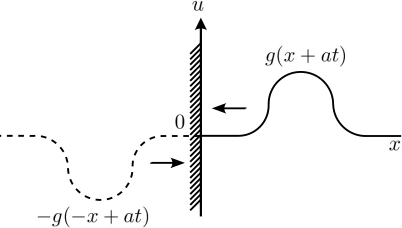
\includegraphics[width=\textwidth]{img/mirror1.png}
		\caption{}
	\end{subfigure}
	\hspace{5mm}
	\begin{subfigure}{0.4\textwidth}
		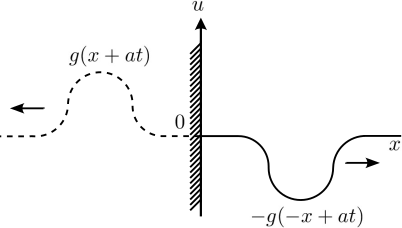
\includegraphics[width=\textwidth]{img/mirror2.png}
		\caption{}
	\end{subfigure}
	\caption{}
\end{figure}
Отсюда из условий \eqref{inf_str_cond} вытекает, что решение $\tilde{u}(x, t)$ удовлетворяет начальным условиям
\begin{equation}
	\tilde{u}|_{t = 0} = \tilde{u}_0(x), \quad \tilde{u}_t|_{t = 0} = \tilde{u}_1(x),
\end{equation}
где $\tilde{u}_0$ и $\tilde{u}_1$ --- нечетные продолжения функций $u_0$ и $u_1$ соответственно. Но решение такой задачи Коши единственно и представляется формулой Даламбера \eqref{dAlamber} с заменой $u_0$ на $\tilde{u}_0$ и $u_1$ на $\tilde{u}_1$, если $\tilde{u}_0 \in \mathcal{C}^2(\mathbb{R}^1)$ и $\tilde{u}_1 \in \mathcal{C}^1(\mathbb{R}^1)$. Последние условия будут выполнены, если
\begin{equation} \label{setcond}
	u_0 \in \mathcal{C}^2(x \geqslant 0), \quad u_1 \in \mathcal{C}^1(x \geqslant 0), \quad u_0(0) = u_0''(0) = u_1(0) = 0.
\end{equation}

Итак, если выполнены условия \eqref{setcond}, то решение задачи \eqref{infinite_string}, \eqref{inf_str_cond}, \eqref{x0cond} существует, единственно и задается формулой 
\begin{equation} \label{formula}
	u(x, t) = \frac{1}{2} [\tilde{u}_0(x + a t) + \tilde{u}_0(x - a t)] + \frac{1}{2 a} \int_{x - a t}^{x + a t} \tilde{u}_1(\xi) \, d\xi, \quad x \geqslant 0.
\end{equation}

Пусть $x - a t \geqslant 0$. Тогда
\begin{equation}
	\tilde{u}_0(x - a t) = \tilde{u}_0(x - a t), \quad \tilde{u}_1(\xi) = u_1(\xi), \quad \xi \geqslant x - a t \geqslant 0,
\end{equation}
и формула \eqref{formula} принимает вид 
\begin{equation}
	u(x, t) = \frac{1}{2} [u_0(x + a t) + u_0(x - a t)] + \frac{1}{2 a} \int_{x - a t}^{x + a t} u_1(\xi) \, d\xi, \quad x \geqslant at.
\end{equation}

Аналогичные рассуждения можно провести для $x - a t \leqslant 0$. 
\begin{equation*}
	\tilde{u}_0(x - a t) = - u_0(-x + a t), \quad \tilde{u}_1(\xi) = -u_1(-\xi), \quad x - a t \leqslant \xi \leqslant 0,
\end{equation*}
формула \eqref{formula} принимает вид
\begin{equation} \label{other_formula}
	u(x, t) = \frac{1}{2} [u_0(x + a t) - u_0(-x + a t)] + \frac{1}{2a} \int_{-x + a t}^{x + a t} u_1(\xi) \,d\xi, \quad 0 \leqslant x \leqslant a t.
\end{equation}

Как видно из формулы \eqref{other_formula}, в точку $(x, t)$, $0 \leqslant x \leqslant a t$, приходят два волны: прямая волна из точки $(x + a t, 0)$ и один раз отраженная волна из точки $(a t - x, 0)$ (совпадающая с прямой волной из фиктивной точки $(x - at, 0)$; см. рис.).

\begin{wrapfigure}{R}{0.5\textwidth}
	\centering
	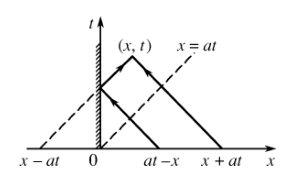
\includegraphics[width=0.9\linewidth]{img/mirror3}
	\caption{}
\end{wrapfigure}

Аналогично рассматривается смешанная задача для полубесконечной струны $x > 0$ со свободным концом:
\begin{equation*}
	u_x|_{x = 0} = 0.
\end{equation*}
Здесь также имеет место отражение волн от конца струны $x = 0$, но уже без изменения знака. 
 \newpage
	\subsection{Энергия колебаний ограниченной струны. Теорема единственности для смешанной краевой задачи для уравнения колебаний струны.}

\paragraph{Энергия колебаний ограниченной струны.}

Найдем выражение для энергии поперечных колебаний струны $E = K + U$, где $K$ --- кинетическая и $U$ - потенциальная энергия. Элемент струны $dx$, движущийся со скоростью $v = u_t$, обладает кинетической энергией 
\begin{equation*}
	\frac{1}{2} m v^2 = \frac{1}{2} \rho(x) (u_t)^2 \, dx \quad (m = \rho \, dx)
\end{equation*}

Кинетическая энергия всей струны равна 
\begin{equation}
	K = \frac{1}{2} \int \limits_{0}^{l} \rho(x) [u_t(x, t)]^2 \, dx.
\end{equation}

Потенциальная энергия поперечных колебаний струны, имеющей при $t = t_0$ форму $u(x, t_0) = u_0(x)$, равна работе, которую надо совершить, чтобы струна перешла из положения равновесия в положение $u_0(x)$. Пусть функция $u(x, t)$ дает профиль струны в момент $t$, причем
\begin{equation*}
	u(x, 0) = 0, \quad u(x, t_0) = u_0(x).
\end{equation*}
Элемент $dx$ под действием равнодействующей сил натяжения 
\begin{equation*}
	T \frac{\partial u}{\partial x} \Big|_{x + dx} - T \frac{\partial u}{\partial x} \Big|_{x} = T u_{xx} \, dx
\end{equation*}
за время $dt$ проходит путь $u_t(x, t) \, dt$. Работа, производимая всей струной за время $dt$, равна
\begin{equation*}
	\Bigg\{\int \limits_{0}^{l} T_0 u_{xx} u_t \, dx \Bigg\} \, dt = \Bigg\{T_0 u_x u_t \Big|_{0}^{l} - \int \limits_{0}^{l} T_0 u_x u_{xt} \, dx \Bigg\} \, dt =  \Bigg\{-\frac{1}{2} \frac{d}{dt} \int \limits_{0}^{l} T_0 (u_x)^2 \, dx + T_0 u_x u_t \Big|_{0}^{l}\Bigg\} \, dt.
\end{equation*}
Интегрируя по $t$ от $0$ до $t_0$, получаем
\begin{equation*}
	-\frac{1}{2} \int \limits_{0}^{l} T_0(u_x)^2 \, dx \Big|_{0}^{t_0} + \int \limits_{0}^{t_0} T_0 u_x u_t \Big|_{0}^{l} \, dt = -\frac{1}{2} \int \limits_{0}^{l} T_0 [u_x(x, t_0)]^2 \, dx + \int \limits_{0}^{t_0} T_0 u_x u_t \Big|_{0}^{l} \, dt.
\end{equation*}

Нетрудно выяснить смысл последнего слагаемого правой части этого равенства. Действительно, $T_0 u_x|_{x = 0}$ есть величина натяжения на конце струны $x = 0; \, u_t(0, t) \, dt$  --- перемещение этого конца, а интеграл 
\begin{equation}
	\int \limits_{0}^{t_0} T_0 u_x u_t|_{x = 0} \, dt
\end{equation}
представляет работу, которую надо затратить на перемещение конца $x = 0$. Аналогичный смысл имеет слагаемое, соответствующее $x = l$. 

Если концы струны закрепленны, то работа на них будет равна нулю (при этом $u(0, t) = 0, u_t(0, t) = 0$). Следовательно, при перемещении закрепленной на концах струны из положения равновесия $u = 0$ в положение $u_0(x)$ работа не зависит от способа перехода струны в это положение и равна 
\begin{equation}
	-\frac{1}{2} \int \limits_{0}^{l} T_0[u'_0(x)]^2 \, dx, 
\end{equation}
потенциальной энергии струны в момент $t = t_0$ с обратным знаком.

Таким образом, полная энергия струны равна
\begin{equation}
	E = \frac{1}{2} \int \limits_{0}^{l} [T_0(u_x)^2 + \rho(x)(u_t)^2] \, dx.
\end{equation}

Совершенно аналогично может быть получено выражение для потенциальной энергии продольных колебаний стержня. Впрочем, его можно получить также, исходя из формулы для потенциальной энергии упругого стержня
\begin{equation*}
	U = \frac{1}{2} k(\frac{l - l_0}{l_0})^2 l_0,
\end{equation*}
где $l_0$ --- начальная длина стержня, $l$ --- конечная длина. Отсюда непосредственно следует 
\begin{equation*}
	U = \frac{1}{2} \int \limits_{0}^{l} k(u_x)^2 \, dx.
\end{equation*}

\paragraph{Теорема единственности для смешанной краевой задачи для уравнения колебаний струны.}

\textit{Возможно существование только одной функции $u(x, t)$, определенной в области $0 \leqslant x \leqslant l, t \geqslant 0$ и удовлетворяющей уравнению}
\begin{align} \label{equa}
	\rho(x) \frac{\partial^2 u}{\partial t^2} = \frac{\partial}{\partial x} \Big(k(x) \frac{\partial u}{\partial x}\Big) + F(x, t) \quad (\rho(x) > 0, k(x) > 0), \\
	0 < x < l, t > 0,
\end{align}
\textit{начальным и граничным условиям}
\begin{equation}
	\begin{rcases}
		u(x, 0) = \varphi(x), \quad u_t(x, 0) = \psi(x), \\
		u(0, t) = \mu_1(t), \quad u(l, t) = \mu_2(t),
	\end{rcases}
\end{equation}
\textit{если выполнены условия:}
\textit{\begin{enumerate}
	\item функция $u(x, t)$ и производные, входящие в уравнение \eqref{equa}, а также производная $u_{xt}$ непрерывны на отрезке $0 \leqslant x \leqslant l$ при $l \geqslant 0$;
	\item коэффициенты $\rho(x)$ и $k(x)$ непрерывны на отрезке $0 \leqslant x \leqslant l$.
\end{enumerate}}

Допустим, что существует два решения $u_1(x, t)$ и $u_2(x, t)$, и рассмотрим разность $v(x, t) = u_1(x, t) - u_2(x, t)$. 

Функция $v(x, t)$, очевидно, удовлетворяет однородному уравнению
\begin{equation} \label{homoeqrho}
	\rho \frac{\partial^2 v}{\partial t^2} = \frac{\partial}{\partial x} \Big(k \frac{\partial v}{\partial x}\Big)
\end{equation}
и однородным дополнительным условиям 
\begin{equation}
	\begin{rcases}
		v(x, 0) = 0, \quad v(0, t) = 0, \\
		v_t(x, 0) = 0; \quad v(l, t) = 0,
	\end{rcases}
\end{equation}
а также условию теоремы.

Докажем, что функция $v(x, t)$ тождественно равна нулю.

Рассмотрим функцию 
\begin{equation}
	E(t) = \frac{1}{2} \int \limits_{0}^{l} [k(v_x)^2 + \rho(v_t)^2] \, dx
\end{equation}
и покажем, что она не зависит от $t$. Продифференцируем $E(t)$ по $t$:
\begin{equation*}
	\frac{d E(t)}{dt} = \int \limits_{0}^{l} (k v_x v_{xt} + \rho v_t v_{tt}) \, dx.
\end{equation*}
Интегрируя по частям первое слагаемое правой части, будем иметь
\begin{equation} \label{firstint}
	\int \limits_{0}^{l} k v_x v_{xt} \, dx = [k v_x v_t]_{0}^{l} - \int \limits_{0}^{l} v_t (k v_x)_x \, dx.
\end{equation}
Подстановка обращается в нуль в силу граничных условий (из $v(0, t) = 0$ следует $v_t(0, t) = 0$ и аналогично для $x = l$). Отсюда
\begin{equation*}
	\frac{d E(t)}{dt} = \int \limits_{0}^{l} [\rho v_t v_{tt} - v_t (k v_x)_x] \, dx = \int \limits_{0}^{l} v_{t} [\rho v_{tt} - (k v_{x})_x] \, dx = 0,
\end{equation*}
т.е. $E(t) = const$. Учитывая начальные условия, получаем
\begin{equation} \label{energ}
	E(t) = const = E(0) = \frac{1}{2} \int \limits_{0}^{l} [k(v_x)^2 + \rho (v_t)^2]_{t = 0} \, dx = 0,
\end{equation}
так как 
\begin{equation*}
	v(x, 0) = 0, v_t(x, 0) = 0.
\end{equation*}

Пользуясь формулой\eqref{energ} и положительностью $k$ и $\rho$, заключаем, что 
\begin{equation*}
	v_x(x, t) \equiv 0, \quad v_t(x, t) \equiv 0,
\end{equation*}
откуда и следует тождество
\begin{equation}
	v(x, t) = const = C_0.
\end{equation}
Исходя из начального условия, находим
\begin{equation*}
	v(x, 0) = C_0 = 0;
\end{equation*}
тем самым доказано, что 
\begin{equation}
	v(x, t) \equiv 0.
\end{equation}

Следовательно, если существует две функции: $u_1(x, t)$ и $u_2(x, t)$, удовлетворяющие всем условиям теоремы, то $u_1(x, t) \equiv u_2(x, t)$.

Для второй краевой задачи функция $v = u_1 - u_2$ удовлетворяет граничным условиям 
\begin{equation}
	v_x(0, t) = 0, \quad v_x(l, t) = 0,
\end{equation}
и подстановка в формуле \eqref{firstint} также образается в нуль. Дальнейшая часть доказательства теоремы остается без изменений.

Для третьей краевой задачи доказательство требует некоторого видоизменения. Рассматривая по-прежнему два решения $u_1$ и $u_2$, получаем для их разности $v(x, t) = u_1 - u_2$ уравнение \eqref{homoeqrho} и граничные условия 
\begin{equation}
	\begin{rcases}
		v_x(0, t) - h_1 v(0, t) = 0 \quad (h_1 \geqslant 0), \\
		v_x(l, t) + h_2 v(l, t) = 0 \quad (h_2 \geqslant 0).
	\end{rcases}
\end{equation}

Представим подстановку в \eqref{firstint} в виде 
\begin{equation}
	[k v_x v_t]_{0}^{l} = - \frac{k}{2} \frac{\partial}{\partial t}[h_2 v^2(l, t) + h_1 v^2(0, t)].
\end{equation}
Интегрируя $\frac{dE}{dt}$ в пределах от нуля до $t$, получаем
\begin{equation}
	E(t) - E(0) = \int \limits_{0}^{t} \int \limits_{0}^{l} v_t[\rho v_{tt} - (k v_x)_x] \, dx \, dt - \frac{k}{2} \{h_2[v^2(l, t) - v^2(l, 0)] + h_1[v^2(0, t) - v^2(0, 0)]\},
\end{equation}
откуда в силу уравнения и начальных условий следует 
\begin{equation}
	E(t) = -\frac{k}{2} [h_2 v^2(l, t) + h_1 v^2(0, t)] \leqslant 0.
\end{equation}

Так как ввиду неотрицательности подынтегральной функции значения $E(t) \geqslant 0$, то 
\begin{equation}
	E(t) \equiv 0,
\end{equation}
а следовательно, и
\begin{equation}
	v(x, t) \equiv 0.
\end{equation}

 \newpage
	\subsection{Метод разделения переменных для уравнения колебаний на отрезке.}

Метод разделения переменных, или метод Фурье является одним из наиболее распространенных методов решения уравнений с частными производными.

Изложение этого метода проведем для задачи колебания струны, закрепленной на концах (т.е. на отрезке). 

Итак, будем искать решение уравнения 
\begin{equation} \label{oscil}
	u_{tt} = a^2 u_{xx},
\end{equation}
удовлетворяющее однородным граничным условиям 
\begin{equation} \label{bord_cond}
	u(0, t) = 0, u(l, t) = 0
\end{equation}
и начальным условиям 
\begin{equation} \label{init_cond}
	\begin{cases}
		u(x, 0) = \varphi(x),
		\\
		u_t(x, 0) = \psi(x).
	\end{cases}
\end{equation}

Уравнение \eqref{oscil} линейно и однородно, поэтому сумма частных решений также является решением этого уравнения. Имея достаточно большое число частных решений, можно попытаться при помощи суммирования их с некоторыми коэффициентами найти искомое решение. 

Поставим основную вспомогательную задачу.

\textit{Найти решение уравнения}
\begin{equation*}
	u_{tt} = a^2 u_{xx},
\end{equation*}
\textit{не равное тождественно нулю, удовлетворяющее однородным граничным условиям}
\begin{equation}
	\label{ucond}
	\begin{cases}
		u(0, t) = 0,
		\\
		u(l, t) = 0
	\end{cases}
\end{equation}
\textit{и представимое в виде произведения}
\begin{equation} \label{sol_form}
	u(x, t) = X(x) T(t),
\end{equation}
\textit{где $X(x)$ --- функция только переменного $x$, $T(t)$ --- функция только переменного $t$.}

Подставляя предполагаемую форму решения \eqref{sol_form} в уравнение \eqref{oscil}, получим 
\begin{equation*}
	X'' T = \frac{1}{a^2} T'' X,
\end{equation*}
или, после деления на $X T$,
\begin{equation} \label{need}
	\frac{X''(x)}{X(x)} = \frac{1}{a^2} \frac{T''(t)}{T(t)}.
\end{equation}

Чтобы функция \eqref{sol_form} была решением уравнения \eqref{oscil}, равенство \eqref{need} должно удовлетворяться тождественно, т.е. для всех значений назависимых переменных $0 < x < l$, $t > 0$. Правая часть равенства \eqref{need} является функцией только переменного $t$, а левая --- только $x$. Фиксируя, например, некоторое значение $x$ и меняя $t$ (или наоборот), получим, что правая и левая части равенства \eqref{need} при изменении своих аргементов сохраняют постоянное значение
\begin{equation} \label{comstlambd}
	\frac{X''(x)}{X(x)} = \frac{1}{a^2} \frac{T''(t)}{T(t)} = -\lambda,
\end{equation}
где $\lambda$ --- постоянная, которую для удобства последующих выкладок берем со знаком "минус", ничего не предполагая при этом о ее знаке.

Из соотношения \eqref{comstlambd} получаем обыкновенные дифференциальные уравнения для определения функций $X(x)$ и $T(t)$:
\begin{align}
	&X''(x) + \lambda X(x) = 0, \quad X(x) \not \equiv 0, \\
	&T''(t) + a^2 \lambda T(t) = 0, \quad T(t) \not \equiv 0. \label{Teq}
\end{align}

Граничные условия \eqref{bord_cond} дают
\begin{align*}
	u(0, t) = X(0) T(t) = 0, \\
	u(l, t) = X(l) T(t) = 0.
\end{align*}
Отсюда следует, что функция $X(x)$ должна удовлетворять дополнительным условиям 
\begin{equation}
	X(0) = X(l) = 0,
\end{equation}
так как иначе мы имели бы
\begin{equation*}
	T(t) \equiv 0 \text{ и } u(x, t) \equiv 0,
\end{equation*}
в то время как задача состоит в нахождении нетривиального решения. Для функции $T(t)$ в основной вспомогательной задаче никаких дополнительных условий нет. 

Таким образом, в связи с нахождением функции $X(x)$ мы приходим к простейшей задаче о собственных значениях.
\begin{equation} \label{euigen}
	\begin{cases} 
		X''(x) + \lambda X(x) = 0, \\
		X(0) = X(l) = 0.
	\end{cases}
\end{equation}

Рассмотрим отдельно возможные значения параметра $\lambda$:
\begin{enumerate}
	\item $\lambda < 0$
	\begin{equation*}
		X(x) = C_1 e^{\sqrt{- \lambda} x} + C_2 e^{-\sqrt{- \lambda} x}.
	\end{equation*}
	Граничные условия дают
	\begin{align*}
		X(0) = C_1 + C_2 = 0, \\
		X(l) = C_1 e^{\alpha} + C_2 e^{-\alpha} = 0 \quad (\alpha = l\sqrt{-\lambda}),
	\end{align*}
	т.е. 
	\begin{equation*}
		C_1 = - C_2 \text{ и } C_1(e^{\alpha} + e^{-\alpha}) = 0.
	\end{equation*}
	Но в рассматриваемом случае $\alpha$ действительно и положительно, так что $e^{\alpha} - e^{-\alpha} \not = 0$. Поэтому 
	\begin{equation*}
		C_1 = C_2 = 0,
	\end{equation*}
	следовательно, 
	\begin{equation*}
		X(x) \equiv 0.
	\end{equation*}
	
	\item $\lambda = 0$
	\begin{equation*}
		X(x) = C_1 x + C_2.
	\end{equation*}
	Граничные условия дают
	\begin{align*}
		X(0) = [C_1 x + C_2]_{x = 0} = C_2 = &~0, \\
		X(l) = C_1 l = &~0,
	\end{align*}
	т.е. $C_1 = 0$ и $C_2 = 0$ и, следовательно, 
	\begin{equation*}
		X(x) \equiv 0. 
	\end{equation*}
	
	\item $\lambda > 0$
	\begin{equation*}
		X(x) = D_1 \cos{\sqrt{\lambda} x} + D_2 \sin{\sqrt{\lambda} x}.
	\end{equation*}
	Граничные условия дают
	\begin{align*}
		X(0) = D_1 = 0, \\
		X(l) = D_2 \sin{\sqrt{\lambda}l} = 0. 
	\end{align*}
	Если $X(x)$ не равно тождественно нулю, то $D_2 \not = 0$, поэтому 
	\begin{equation*}
		\sin{\sqrt{\lambda}l} = 0,
	\end{equation*}
	или
	\begin{equation*}
		\sqrt{\lambda} = \frac{\pi n}{l},
	\end{equation*}
	где $n$ --- любое целое число. Следоовательно, нетривиальные решения задачи \eqref{euigen} возможны лишь при значениях 
	\begin{equation*}
		\lambda = \lambda_n = \Big(\frac{\pi n}{l}\Big)^2.
	\end{equation*}
	Этим собственным значениям соответствуют собственные функции \begin{equation*}
		X_n(x) = D_n \sin{\frac{\pi n}{l} x},
	\end{equation*}
	где $D_n$ --- произвольная постоянная.
	
	
	Итак, только при значениях $\lambda$, равных
	\begin{equation*}
		\lambda_n = \Big(\frac{\pi n}{l}\Big)^2.
	\end{equation*}
	существуют нетривиальные решения задачи \eqref{euigen}
	\begin{equation*}
		X_n(x) = \sin{\frac{\pi n}{l} x},
	\end{equation*}
	определяемые с точностью до произвольного множителя, который мы положили равным единице. Этим же значениям $\lambda_n$ соответствуют решения уравнения \eqref{Teq}
	\begin{equation*}
		T_n(t) = A_n \cos{\frac{\pi n}{l} a t} + B_n \sin{\frac{\pi n}{l} a t},
	\end{equation*}
	где $A_n$ и $B_n$ --- произвольные постоянные.
\end{enumerate}
	
Возвращаясь к задаче \eqref{oscil}---\eqref{init_cond} заключаем, что функции 
	\begin{equation*}
		u_n(x, t) = X_n(x) T_n(t) = \Big(A_n \cos{\frac{\pi n}{l} a t} + B_n \sin{\frac{\pi n}{l} a t}\Big) \sin{\frac{\pi n}{l} x}
	\end{equation*}
	являются частными решениями уравнения \eqref{oscil}, удовлетворяющими граничными условиям \eqref{ucond} и представивым в виде произведения \eqref{sol_form}. Эти решения могут удовлетворить начальным условиям \eqref{init_cond} нашей задачи только для частных случаев начальных функций $\varphi(x)$ и $\psi(x)$.
	
	Обратимся к решению задачи \eqref{oscil}---\eqref{init_cond} в общем случае 
	\begin{equation} \label{sol}
		u(x, t) = \sum \limits_{n = 1}^{\infty} u_n(x, t) = \sum \limits_{n = 1}^{\infty} \Big(A_n \cos{\frac{\pi n}{l} a t} + B_n \sin{\frac{\pi n}{l} a t}\Big) \sin{\frac{\pi n}{l} x}
	\end{equation} 
	В силу линейности оно также удовлетворяет граничным условиям. Начальные условия позволят определить коэффициенты $A_n$ и $B_n$.
	\begin{equation} \label{formulas}
		\begin{cases}
			u(x, 0) = \varphi(x) = \sum \limits_{n = 1}^{\infty} u_n(x, 0) = \sum \limits_{n = 1}^{\infty} A_n \sin{\frac{\pi n}{l} x}, \\
			u_t(x, 0) = \psi(x) = \sum \limits_{n = 1}^{\infty} \frac{\partial u_n}{\partial t}(x, 0) = \sum \limits_{n = 1}^{\infty} \frac{\pi n}{l} a B_n \sin{\frac{\pi n}{l} x}.
		\end{cases}
	\end{equation}
	Из теории рядов Фурье известно, что произвольная кусочно-непрерывная и кусочно-дифференцируемая функция $f(x)$, заданная в промежутке $0 \leqslant x \leqslant l$, разлагается в ряд Фурье
	\begin{equation}
		f(x) = \sum \limits_{n = 1}^{\infty} b_n \sin{\frac{\pi n}{l} x},
	\end{equation}
	где
	\begin{equation}
		b_n = \frac{2}{l} \int \limits_{0}^{l} f(\xi) \sin{\frac{\pi n}{l}\xi} \, d\xi. 
	\end{equation}
	Если функции $\varphi(x)$ и $\psi(x)$ удовлетворяют условиям разложения в ряд Фурье, то
	\begin{align}
		\varphi(x) = \sum \limits_{n = 1}^{\infty} \varphi_{n} \sin{\frac{\pi n}{l} x}, \quad \varphi_n = \frac{2}{l} \int \limits_{0}^{l} \varphi(\xi) \sin{\frac{\pi n}{l} \xi} \, d\xi, \\
		\psi(x) = \sum \limits_{n = 1}^{\infty} \psi_{n} \sin{\frac{\pi n}{l} x}, \quad \psi_n = \frac{2}{l} \int \limits_{0}^{l} \psi(\xi) \sin{\frac{\pi n}{l} \xi} \, d\xi.
	\end{align}
	
	Сравнение этих рядов с формулами \eqref{formulas} показывает, что для выполнения начальных условий надо положить 
	\begin{equation}
		A_n = \varphi_n, \quad B_n = \frac{l}{\pi n a} \psi_n,
	\end{equation}
	чем полностью определяется функция \eqref{sol}, лающая решение исследуемой задачи.  \newpage
	\subsection{Смешанная краевая задача о колебаниях прямоугольной мембраны. Метод разделения переменных.}

Процесс колебаний плоской однородной мембраны описывается уравнением колебаний 
\begin{equation} \label{memb_prob}
	u_{tt} = a^2 \Delta u.
\end{equation}

Пусть в плоскости $(x, y)$ расположена прямоугольная мембрана со сторонами $b_1$ и $b_2$, закрепленная по краям и возбуждаемая с помощью начального отклонения и начальной скорости. Для нахождения функции $u(x, y, t)$, характеризующей отклонение мембраны от положения равновесия, мы должны решить уравнение колебаний 
\begin{equation}
	\tag{77'}
	\frac{\partial^2 u}{\partial t^2} = a^2 \Bigg(\frac{\partial^2 u}{\partial x^2} + \frac{\partial^2 u}{\partial y^2}\Bigg)
\end{equation}
при заданных начальных условиях 
\begin{equation} \label{init_cond_memb}
	\begin{cases}
		u(x, y, 0) = \varphi(x, y), \\
		\frac{\partial u}{\partial t}(x, y, 0) = \psi(x, y)
	\end{cases}
\end{equation}
и граничных условиях
\begin{align}
	u(0, y, t) = 0, \quad u(b_1, y, t) = 0, \\
	u(x, 0, t) = 0, \quad u(x, b_2, t) = 0. \label{bord_cond_memb}
\end{align}

Мы ищем решение методом Фурье, полагая
\begin{equation} \label{fourie_sol_memb}
	u(x, y, t) = v(x, y) T(t).
\end{equation}

Подставляя \eqref{fourie_sol_memb} в \eqref{memb_prob} и разделяя переменные получаем для $T(t)$
\begin{equation}
	T'' + a^2 \lambda T = 0,
\end{equation}
а для $v(x, y)$ --- следующую краевую задачу:
\begin{equation}
	\begin{cases}
		v_{xx} + v_{yy} + \lambda v = 0; \\
		v(0, y) = 0, \quad v(b_1, y) = 0 \\
		v(x, 0) = 0, \quad v(x, b_2) = 0.
	\end{cases}
\end{equation}

Таким образом, сама задача ждя собственных значений состоит в решении однородного уравнения в частных производных при однородных граничных условиях. Будем и эту задачу решать методом разделения переменных, полагая 
\begin{equation*}
	v(x, y) = X(x) Y(y)
\end{equation*}

Проводя разделение переменных получаем следующие одномерные задачи на собственные значения 
\begin{align}
	\begin{cases}
		X'' + \nu X = 0, \\
		X(0) = 0, \quad X(b_1) = 0;
	\end{cases} \label{Xprob}\\
	\begin{cases}
		Y'' + \mu Y = 0, \\
		Y(0) = 0, \quad Y(b_2) = 0,
	\end{cases} \label{Yprob}
\end{align}
где $\mu$ и $\nu$ связаны соотношением $\mu + \nu = \lambda$. 

Решения уравнений \eqref{Xprob} и \eqref{Yprob} имеют вид
\begin{gather*}
	X_n(x) = \sin{\frac{n \pi}{b_1} x}, \quad Y_{m}(y) = \sin{\frac{m \pi}{b_2} y}; \\
	\nu_n = \Big(\frac{n \pi}{b_1}\Big)^2; \quad \mu_m = \Big(\frac{m \pi}{b_2}\Big)^2.
\end{gather*}
Собственным значениям 
\begin{equation*}
	\lambda_{n, m} = \Big(\frac{n \pi}{b_1}\Big)^2 + \Big(\frac{m \pi}{b_2}\Big)^2;
\end{equation*}
таким образом, соответствуют собственные функции
\begin{equation*}
	v_{n, m} = A_{n, m} \sin{\frac{n \pi}{b_1} x} \sin{\frac{m \pi}{b_2} y},
\end{equation*}
где $A_{n, m}$ --- некоторый постоянный множитель. Выберем его так, чтобы норма функции $v_{m, n}$ была равне единице:
\begin{equation*}
	\int \limits_{0}^{b_1} \int \limits_{0}^{b_2} v^2_{n, m} \, dx \, dy = A_{n, m}^2 \int \limits_0^{b_1} \sin^2{\frac{n \pi}{b_1}x} \, dx \int \limits_{0}^{b_2} \sin^2{\frac{m \pi}{b_2} y} \, dy = 1 \Rightarrow A_{n, m} = \sqrt{\frac{4}{b_1 b_2}}.
\end{equation*}
Функции
\begin{equation} \label{Vformula}
	v_{n, m}(x, y) = \sqrt{\frac{4}{b_1 b_2}} \sin{\frac{n \pi}{b_1} x} \sin{\frac{m \pi}{b_2} y}
\end{equation}
образуют ортонормированную систему собственных функций прямоугольной мембраны.

Возвращаясь к исходной задаче для уравнения \eqref{memb_prob}, мы видим, что частные решения
\begin{equation}
	u_{n, m} = v_{n, m}(x, y) \underbrace{C_{n, m} \cos{\sqrt{\lambda_{n, m}} a t} + D_{n, m} \sin{\sqrt{\lambda_{n, m}} a t}}_{=T(t)}
\end{equation}
представляют собой стоячие волны, профиль которых определяется собственными функциями $v_{n, m}$. Геометрические места точек внутри прямоугольника, в которых собственные функции обращаются в нуль, называют узловыми линиями. Расмотрим для простоты квадрат со стороной $b (b_1 = b_2)$. Узловые линии функции 
\begin{equation}
	v_{n, m} = \frac{2}{b} \sin{\frac{n \pi}{b} x} \sin{\frac{m \pi}{b} y}
\end{equation}
являются прямыми, параллельными осям координат. 

Искомое решение уравнения \eqref{memb_prob} при дополнительных условиях \eqref{init_cond_memb}---\eqref{bord_cond_memb} имеет вид
\begin{equation*}
	u(x, y, t) = \sum \limits_{m = 1}^{\infty} \sum \limits_{n = 1}^{\infty} ()
\end{equation*}
где $v_{n, m}$ определяется формулой \eqref{Vformula}, а коэффициенты $C_{n, m}$ и $D_{n, m}$ равны
\begin{align*}
	&C_{n, m} = \int \limits_{0}^{b_1} \int \limits_{0}^{b_2} \varphi(x, y) v_{n, m}(x, y) \, dx \, dy = \sqrt{\frac{4}{b_1 b_2}} \int \limits_{0}^{b_1} \int \limits_{0}^{b_2} \varphi(x, y) \sin{\frac{n \pi}{b_1} x} \sin{\frac{m \pi}{b_2} y} \, dx \, dy, \\
	&D_{n, m} = \frac{1}{\sqrt{a^2 \lambda_{n, m}}} \sqrt{4}{b_1 b_2} \int \limits_{0}^{b_1} \int \limits_{0}^{b_2} \psi(x, y) \sin{\frac{n \pi}{b_1} x} \sin{\frac{m \pi}{b_2} y} \, dx \, dy. 
\end{align*} \newpage
	\subsection{Распространение тепла в стержне. Постановка смешанной краевой задачи}
\subsection*{Уравнение теплопроводности в стержне}
Простейшее уравнение параболического (см. \ref{sec:types}) типа 
\begin{equation}
  \label{eq:teplo_eq}
  u_{xx} - u_y = 0, \quad y = a^2t,
\end{equation}
то есть 
\[
  u_t = a^2u_{xx},
\]
обычно называют \emph{уравнением теплопроводности}.

Рассмотрим стержень длины $ l $, теплоизолированный с боков и 
достаточно тонкий, чтобы в любой момент времени температуру во всех 
точках поперечного сечения можно было считать одинаковой. Концы стержня будем
поддерживать при постоянных температурах $ u_1 $ и $ u_2 $. Как известно (?),
вдоль стержня тогда установится линейной распределение температуры, то есть
функция температуры имеет вид
\[
  u(x) = u_1 + \frac{u_2 - u_1}{l}x,
\]
где, например, $ u_1 > u_2 $.

Тепло\footnote{То есть энергия теплового электро-магнитного излучения.} течёт от $ u_1 $ к $ u_2 $. Экспериментальный факт: количество тепла,
протекающего через сечение\footnote{Здесь и далее имеется в виду поперечное
сечение (?).} стержня площади $ S $ за единицу времени равно 
\begin{equation}
  \label{eq:potok}
  Q = -k \frac{u_2 - u_1}{l} S = -k \frac{\partial u}{\partial x}S,
\end{equation}
где $ k $ --- коэффициент теплопроводности, зависящий от материала
стержня. Изучив конечный результат процесса, попробуем изучить сам процесс
распространения тепла в стержне.
\begin{enumerate}
  \item \textsc{Закон Фурье.} Обобщим формулу \eqref{eq:potok}. Количество
    тепла, протекающее через сечение $ x $ за промежуток
времени $ (t_1, t_2) $, равно 
\begin{equation}
  \label{eq:fourier}
  % dQ = qS\,dt,
  Q = -S\int\limits_{t_1}^{t_2}k(x) \frac{\partial u}{\partial x}(x, t)\,dt.
\end{equation}
% где 
% \[
%     q = -k(x) \frac{\partial u}{\partial x}
% \]
% --- \emph{плотность теплового потока}, то есть количество тепла, проходящего за
% единицу времени\footnote{Время бесконечно малое, а
% площадь --- нет.} через площадь в 1\,см$^2$. 
В общем случае неоднородного стержня
коэффициент $ k $ является функцией от $ x $. 
% Закон \eqref{eq:fourier} можно также записать и
% в интегральной форме.
\item Количество тепла, которое нужно сообщить стержню, чтобы повысить его
  температуру $ \Delta u(x) $, равно  
  \begin{equation}
    \label{eq:2}
    Q =\int\limits_{x_1}^{x_2} c\rho(x) S\Delta u(x)\,dx,
  \end{equation}
  где $ c $ --- удельная теплоёмкость, $ \rho(x) $ --- плотность неоднородного в
  общем случае тела. При постоянных $ \rho $, $ \Delta u $ формула упрощается до
  $ Q = cm\Delta u $.
\item Внутри стержня тоже может возникать или поглощаться тепло (например, при
  прохождении тока, химических реакций и т.\,д.). Если известна объёмная
  плотность $ F(x, t) $ внутренних тепловых источников, то выделяемое ими тепло
  на промежутке $ (x_1, x_2) $ за время $ (t_1, t_2) $
  равно 
  \begin{equation}
    \label{eq:F}
    Q = S\int\limits_{t_1}^{t_2}\int\limits_{x_1}^{x_2}F(t, x)\,dx\,dt.
  \end{equation}
\end{enumerate}
  
Применим к отрезку $ (x_1, x_2) $ и промежутку времени $ (t_1, t_2) $ закон
сохранения энергии и формулы \eqref{eq:fourier}, \eqref{eq:2}, \eqref{eq:F}, и
получим 
\[
 \int\limits_{t_1}^{t_2} \left[\left. k \frac{\partial u}{\partial
   x}(x,\tau)\right|_{x=x_2} -\left. k \frac{\partial u}{\partial x}(x,
   \tau)\right|_{x=x_1} \right] \,d\tau
   +\int\limits_{x_1}^{x_2}\int\limits_{t_1}^{t_2} F(\xi, \tau)\,d\xi\,d\tau =
     \int\limits_{x_1}^{x_2}c\rho[u(\xi, t_2) - u(\xi, t_1)]\,d\xi
\]
--- уравнение теплопроводности в интегральной форме.

Предположим, что функция
$ u(x, t) $ имеет непрерывные производные $ u_{xx} $ и $ u_t $.
Пользуясь сначала интегральной теоремой о среднем, 
\[
  \left[ \left. k \frac{\partial u}{\partial x}(x,\tau) \right|_{x=x_2} -\left.
        k \frac{\partial u}{\partial x}(x,
      \tau)\right|_{x=x_1}  \right]_{\tau=t_3}\Delta t + F(x_4, t_4) \Delta x
      \Delta t = 
      \left\{ c\rho [u(\xi, t_2) - u(\xi, t_1)] \right\}_{\xi = x_3} \Delta x,
\]
а затем дифференциальной теоремой (Лагранжа) о среднем, 
\[
    \frac{\partial}{\partial x} \left[ k \frac{\partial u}{\partial x}(x, t)
    \right]_{\substack{x = x_5 \\ t = t_3}} \Delta x \Delta t + F(x_4, t_4)\Delta x \Delta
    t = \left[ c\rho \frac{\partial u}{\partial t}(x, t)
    \right]_{\substack{x=x_3\\t=t_5}}\Delta x \Delta t,
\]
где $ t_3$, $t_4$, $t_5 $ и $ x_3 $, $ x_4 $, $ x_5 $ --- промежуточные точки
соответствующих интервалов.
Отсюда  
\[
    \frac{\partial }{\partial x} \left.\left( k \frac{\partial u}{\partial x}
        \right)\right|_{\substack{x=x_5 \\ t=t_3}} + \left.F(x,
          t)\right|_{\substack{x=x_4\\t=t_4}} =
          \left. c\rho \frac{\partial u}{\partial t}\right|_{\substack{t=t_5 \\
            x= x_3}}.
\]
Поскольку все рассуждения относились к произвольным промежуткам $ (x_1, x_2) $,
$ (t_1, t_2) $, то устремив $ x_1 $, $ x_2  \to x$ и $ t_1 $, $ t_2 \to t $,
получим уравнение  
\[
    \boxed{\frac{\partial }{\partial x} \left( k \frac{\partial u}{\partial x} \right)
    + F(x, t) = c\rho \frac{\partial u}{\partial t},}
\]
называемое \emph{уравнением теплопроводности}. 

\paragraph{Частные случаи.} Рассмотрим некоторые частные случаи.
\begin{enumerate}
  \item В случае однородного
стержня (постоянства всех коэффициентов) приходим к уравнению
\eqref{eq:teplo_eq}.

 \item Если боковые стенки проводят тепло, то согласно \emph{закону Ньютона}
количество тепла, которое потеряет стержень на единицу длины и времени, равно 
\[
    F_0 = h(u - \theta),
\]
где $ \theta(x, t) $ --- температура окружающей среды, $ h $ --- коэффициент
теплообмена. Тогда $ F(x, t) = F_1(x, t) - F_0 $ (где $ F_1 $ --- объёмная
плотность источников тепла), и в случае однородности
стержня 
\[
  u_t = a^2 u_{xx} - \alpha u + f(x, t),
\]
где $ \alpha = h/(c\rho) $, $ f(x, t) = \alpha\theta(x, t) + F_1/(c\rho) $.

\item  Коэффициенты $ k $ и $ c $ медленно зависят от температуры. Предположение об
их постоянстве обусловленно предполагаемым небольшим изменением температуры.
В ином случае уравнение станет квазилинейным.
\end{enumerate}

\subsection*{Постановка смешанной краевой задачи}
Начальное условие задаёт лишь значение функции $ u(x, t) $ в начальный момент
времени $ t_0 $.

Рассматривают три основных типа граничных условий. Любая их комбинация будет
отдельной задачей.
\begin{enumerate}
  \item На конце стержня $ x = 0 $ задана
    температура  
    \[
        u(0, t) = \mu(t)
    \]
    как функция времени.
  \item На конце\footnote{Дело в том, что, как и прежде, подразумевается, что
    тепло идёт слева направо} $ x = l $ задано значение пространственной производной 
  \[
      \frac{\partial u}{\partial x}(l, t) = \nu(t).
  \]
  К такому условию приходим, если известен торцевой тепловой поток (см. формулу
  закона Фурье
  \eqref{eq:fourier}).
  % \[
      %Q(0, t) = -k \frac{\partial u}{\partial x}(0, t).
  % \]
\item На конце $ x = l $ задано линейное соотношение между производной и функцией 
\[
  \frac{\partial u}{\partial x}(l, t) = -\lambda [u(l, t) - \theta(t)].
\]
Этот тип соответствует теплообмену по закону Ньютона. Действительно, приравнивая
плотность излучения внешнего источника (по закону Фурье) и плотность ухода тепла
(по закона Ньютона), получаем исходное граничное условие.
\end{enumerate}

Перечислим некоторые особые случаи. Пусть на конце $ x = 0 $ помещена
сосредоточенная теплоёмкость $ C_1 $ и происходит теплообмен с окружающей средой
по закону Ньютона. Такой закон теплового баланса можно записать в виде условия
\[
    C_1 \frac{\partial u}{\partial t} = k \frac{\partial u}{\partial x} -
    h(u-u_0),
\]
где $ u_0 $ --- температура внешней среды.

%TODO: неоднородная среда

Помимо перечисленных выше линейных задач, ставятся и нелинейные --- например, при
излучении торца по закону \emph{Стефана -- Больцмана} 
\[
  k \frac{\partial u}{\partial x}(0, t) = \sigma [u^4(0, t) - \theta^4(0,t)],
\]
где $ \theta $ --- температура окружающей среды, а $ \sigma $ --- постоянная
Стефана -- Больцмана.

Дополнительным условием для решения будет его непрерывность в соответствующей
замкнутой области. Функция $ u $ обязана удовлетворять уравнению лишь внутри фазового прямоугольника, то
есть при $ 0 < x < l $, $ 0 < t < T $. Требование непрерывности $ u
$ нужно для этих граничных точек, внутри она непрерывна согласно самому уравнению.

\paragraph{Предельные случаи.}\label{sec:teplo} В очень длинном стержне граничные условия в
течение малого промежутка времени влияют на середину стержня очень слабо.
Поэтому их можно опустить, считая стержень бесконечным.

Стержень можно считать и полубесконечным, опуская с такими же рассуждениями одно
из граничных условий, если интересующий нас участок находится близко к одному
концу и очень далеко от другого.

Опустить можно и начальные условия, если считать, что с начала распространения
тепла прошло очень много времени. Тогда считаем, что опыт длится бесконечно.
Часто, например, в подобных задачах граничные
условия периодические: $ \mu(t) = A\cos\omega t $.


 \newpage
	\subsection{Принцип максимального значения для параболического уравнения и теорема единственности смешанной краевой задачи в ограниченной области}
\begin{theorem}[о максимальном значении] Функция $ u(x, t) $, которая на промежутках $ 0 < x < l $, $ 0 <
  t \leqslant T$ удовлетворяет уравнению
\begin{equation}
  \label{eq:9/teplo_eq}
  u_t = a^2u_{xx},
\end{equation}
определённая и непрерывная внутри соответствующей замкнутой области, принимает максимальное и минимальное значения либо в начальный момент, либо в
точке границы $ x = 0 $ или $ x = l $.\end{theorem}

Физический смысл этой теоремы очевиден: если
температура на
границе и в начальный момент не превосходит некоторого значения
$ M $, то при отсутствии источников внутри тела не может создаваться
температура, б\'{о}льшая $ M $. Остановимся сначала на доказательстве
теоремы для максимального значения.

\begin{proof}Пойдём от противного. Обозначим через $ M $ максимум функции в указанных трёх
множествах: $ t = 0 $, $ x = 0 $ и $ x = l $. Предположим, что есть такая
точка\footnote{Такая точка должна существовать, поскольку функция непрерывна на компакте.}
$ (x_0, t_0) $, не принадлежащая перечисленным множествам, где $ u(x, t) $
достигает своего максимума, то есть 
\[
    u(x_0, t_0) = M + \varepsilon, \quad \varepsilon > 0.
\]
Чтобы прийти к противоречию, найдём такую точку $ (x_1, t_1) $, в которой
(вопреки уравнению \eqref{eq:9/teplo_eq}) $ u_{xx} \leqslant 0 $, $ u_t > 0 $.
Воспользуемся вспомогательной функцией  
\[
    v(x, t) := u(x, t) + k(t_0 - t).
\]
Выберем $ 0 < k < \varepsilon/(2T) $. Тогда во всех трёх множествах $
v(x, t) \leqslant M + \varepsilon/2 $. Тогда максимум функции $ v $ достигается
где-то ещё, поскольку хотя бы $ v(x_0, t_0) = M + \varepsilon $, --- в точке,
которую назовём $ (x_1, t_1) $.
Перечислим некоторые необходимые условия этого события\footnote{Действительно,
  будь вторая производная строго больше нуля, то получили бы локальный минимум функции; производная по времени, конечно, может быть больше нуля только в точке $ T $.}: 
\begin{gather*}
    \frac{\partial v}{\partial x}(x_1, t_1) = 0, \quad \frac{\partial^2
    v}{\partial x^2}(x_1, t_1) = \frac{\partial^2 u}{\partial x^2}(x_1, t_1) \leqslant 0,\\
    \frac{\partial v}{\partial t}(x_1, t_1) = \frac{\partial u}{\partial t}(x_1,
    t_1) - k \geqslant 0,
\end{gather*}
откуда и следует доказываемое.
\end{proof}
Чтобы доказать аналогичную теорему для минимального значения, достаточно перейти
к функции $ -u $.

\begin{theorem}[единственности]
  Если две функции $ u_1 $ и $ u_2 $, определённые и непрерывные в области $
  0\leqslant x\leqslant l $, $ 0 \leqslant t \leqslant T $, удовлетворяют
  уравнению теплопроводности  
  \[
    u_t = a^2 u_{xx} + f(x, t), \quad 0 < x < l, \ 0 < t \leqslant T,
  \]
  одинаковым начальным и граничным условиям  
  \begin{align*}
    u_1(x, 0) &= u_2(x, 0) = \varphi(x),\\
    u_1(0, t) &= u_2(0, t) = \mu_1(t),\\
    u_1(l, t) &= u_2(l, t) = \mu_2(t),
  \end{align*}
  то $ u_1 = u_2 $.
\end{theorem}

\begin{proof}
  Рассмотрим функцию $ v = u_2 - u_1 $, которая, конечно, является решением
  соответствующего однородного уравнения. Применяя принцип максимального
  значения к этой функции, приходим к завершению доказательства.
\end{proof}
  
 \newpage
	\subsection{Разделение переменных в смешанной краевой задаче для уравнения теплопроводности/диффузии.
Построение функции влияния мгновенного точечного источника.}

\paragraph{Однородная правая часть} Рассматривается смешанная краевая задача для уравнения
теплопроводности:
\begin{equation}\label{1.10-main-homogeneous}
  \begin{cases}
    u_t = a^2 u_{xx}, \\
    \left. \left( \alpha_1 u + \beta_1 u_x \right) \right|_{x=0} = 0, \\
    \left. \left( \alpha_2 u + \beta_2 u_x \right) \right|_{x = l} = 0, \\
    u(x, 0) = \varphi(x), \\
  \end{cases}
\end{equation}
в которой разделим переменные: $u = X(x) T(t)$:
\[
  \begin{cases}
    \dfrac{1}{a^2} \dfrac{T'}{T} = \dfrac{X''}{X} = - \lambda, \\
    \left( \alpha_1 X(0) + \beta_1 X'(0) \right) T(t) = 0, \\
    \left( \alpha_2 X(l) + \beta_2 X'(l) \right) T(t) = 0. \\
  \end{cases}
\]

Для $X(x)$ получается такая задача:
\[
  \begin{cases}
    -X'' - \lambda X = 0, \\
    \left( \alpha_1 X(0) + \beta_1 X'(0) \right) = 0, \\
    \left( \alpha_2 X(l) + \beta_2 X'(l) \right) = 0,
  \end{cases}
\]
разрешая которую, получим систему функций $X_n$ и соотвествующие собственные значения
$\lambda_n$. Таким образом, решение представляется в виде ряда:
\[
  u(x, t) = \sum_n T_n(t) X_n(x)
\]

Для $T(t)$ тогда:
\[
  \begin{cases}
    - T_n' - a^2 \lambda_n T_n = 0, \\ 
    T_n(0) = \varphi_n,
  \end{cases}
\]
где $\varphi_n$ -- коэффициенты разложения Фурье соответствующей функции.
Общее решение этого диффура представляет собой $T_n = \varphi_n e^{- a^2 \lambda_n t}$, тогда
окончательный ответ:
\[
  u(x, t) = \sum_n \varphi_n e^{ a^2 \lambda_n t} X_n(x)
  = \sum_n
    \left( \dfrac{1}{\|X_n\|^2} \int\limits_0^l \varphi(\xi) X_n(\xi) \, d\xi \right)
    e^{- a^2 \lambda_n t} X_n(x) =
\]
по свойствам линейности и при выполнении условия равномерной сходимости:
\[
  = \int\limits_0^l
    \left( \sum_n \dfrac{1}{\|X_n\|^2} e^{- a^2 \lambda_n t} X_n(\xi) X_n(x) \right)
    \varphi(\xi) \, d\xi
  = \int\limits_0^l G(x, \xi, t) \varphi(\xi) \, d\xi,
\]
а функцию $G = \sum_n \dfrac{1}{\|X_n\|^2} e^{- a^2 \lambda_n t} X_n(\xi) X_n(x)$ называют
\emph{функцией влияния мгновенного точечного источника}.

\paragraph{Неоднородная правая часть} Если в задачу \eqref{1.10-main-homogeneous} добавить 
неоднородность правой части:
\begin{equation}
  \begin{cases}
    u_t = a^2 u_{xx} + f(x, t), \\
    \left. \left( \alpha_1 u + \beta_1 u_x \right) \right|_{x=0} = 0, \\
    \left. \left( \alpha_2 u + \beta_2 u_x \right) \right|_{x = l} = 0, \\
    u(x, 0) = \varphi(x), \\
  \end{cases}
\end{equation}
то решение изменится только на этапе нахождения коэффициентов $T_n(t)$:
\[
  \begin{cases}
    T_n' = - a^2 \lambda_n T_n + f_n(t)
      \Leftrightarrow
      -T_n'(t) - a^2 \lambda_n T_n(t) = - f_n(t), \\
    T_n(0) = 0,
  \end{cases}
\]
где $f_n = \dfrac{1}{\|X_n\|^2} \int_0^l f_n(\xi) X_n(\xi) \, d\xi$ -- коэффициенты разложения
функции $f$. Причём решение представим в виде $T_n(t) = C_n(t) \cdot e^{-a^2 \lambda_n t}$
(метод вариации произвольных постоянных. Тогда несложно получить, что
$C_n(t) = \int_0^t f_n(\tau) e^{a^2 \lambda_n \tau} \, d\tau + C$, подставляя это в начальное
условие, получим что $C = \varphi_n$. Собирая всё вместе:
\begin{multline*}
  u(x, t)
  = \sum_n \left( \varphi_n + \int_0^t f_n(\tau) e^{a^2 \lambda_n \tau} \, d\tau \right) X_n(x) = \\
  = \sum_n \left( \int_0^l \varphi(\xi) X_n(\xi) \, d\xi
    + \int_0^t \left( \int_0^l f(\xi, \tau) X_n(\xi) \dfrac{1}{\| X_n \|^2} \, d\xi 
    \right) e^{a^2 \lambda_n \tau} \, d\tau \right) X_n(x) = \\
  = \int_0^l G(x, \xi, t) \varphi(\xi) \, d\xi
  + \int_0^l \int_0^t \sum_n \dfrac{1}{\|X_n\|^2} X_n(x) X_n(\xi) e^{-a^2 \lambda_n (t-\tau)} f(\xi, \tau) \, d\tau d\xi = \\
  = \int_0^l G(x, \xi, t) \varphi(\xi) \, d\xi
    + \int_0^l \int_0^t G(x, \xi, t-\tau) f(\xi, \tau) \, d\tau d\xi.
\end{multline*}
 \newpage
	\subsection{Уравнение теплопроводности/диффузии на бесконечной и полубесконечной прямой.
Функция влияния мгновенного точечного источника.}

\paragraph{Бесконечная прямая}
\begin{equation}\label{1.10.1-main}
  \begin{cases}
    u_t = a^2 u_{xx} + f(x, t), &-\infty < x < +\infty, t > 0, \\
    |u(\pm \infty, t)| < \infty, \\
    u(x, 0) = \varphi(x),
  \end{cases}
\end{equation}
а теперь проделаем разделение переменных, причём <<переменную разделения>> обозначим за $\lambda^2$,
потому что несложно проверить, что при отрицательных значениях не будет органиченности на
бесконечности. После разделения переменных получаем такую задачу для $X(x)$:
\[
  \begin{cases}
    -X'' - \lambda^2 X = 0, \\
    |X(\pm \infty)| < \infty,
  \end{cases}
\]
несложно получить, что собственные значения такой задачи имеют непрерывный спектр
$\lambda \in (-\infty, +\infty)$, а собственные функции: $X = e^{i\lambda x}$.

Это всё позволяет сказать о общем виде будущего решения:
\[
  u(x, t) = \int\limits_{-\infty}^{+\infty} A(t, \lambda) e^{i \lambda x} \, d\lambda,
\]
подставим это в \eqref{1.10.1-main}:
\[
  \begin{cases}
    \int\limits_{-\infty}^{+\infty} \dfrac{\partial A(t, \lambda)}{\partial t} e^{i \lambda x} \, d\lambda
      = \int\limits_{-\infty}^{+\infty} - a^2 \lambda^2 A(t, \lambda) e^{i \lambda x} \, d\lambda
      + \int\limits_{-\infty}^{+\infty} F(t, \lambda) e^{i \lambda x} \, d\lambda, \\
    
    \int\limits_{-\infty}^{+\infty} A(0, \lambda) e^{i \lambda x} \, d\lambda 
      = \int\limits_{-\infty}^{+\infty} \Phi(\lambda) e^{i \lambda x} \, d\lambda,
  \end{cases}
\]
где $F, \Phi$ -- соответсвующие коэффициенты разложения по базису, а по совместительству -- образы 
преобразования Фурье.

\[
  \begin{cases}
    \dfrac{\partial A(t, \lambda)}{\partial t}
      = - a^2 \lambda^2 A(t, \lambda)
      + F(t, \lambda), \\
    A(0, \lambda) = \Phi(\lambda),
  \end{cases}
\]
такой диффур решим, аналогично такому же диффуру в \ref{question:split-variables-in-heat}, то
есть методом вариации произвольных постоянных. Тогда ответ получим в виде:
\[
  A(t, \lambda) = \left(
    \Phi(\lambda)
    + \int\limits_0^t F(\tau, \lambda) e^{a^2 \lambda^2 \tau} \, d\tau \right)
    \cdot e^{- a^2 \lambda^2 t}
\]
теперь всё что остаётся это найти $F$ и $\Phi$, а их можно найти с помощью обратного преобразования
Фурье:
\[
  f(x, t) = \int\limits_{-\infty}^{+\infty} F(t, \lambda) e^{i \lambda x} \, d\lambda
  \Leftrightarrow
  F(t, \lambda)
  = \dfrac{1}{2\pi} \int\limits_{-\infty}^{+\infty} f(\xi, t) e^{-i \lambda \xi} \, dx,
\]
и аналогично для $\Phi$. Тогда окончательный ответ перепишем в виде:
\begin{multline*}
  u(x, t) = \int\limits_{-\infty}^{+\infty}
    \left( \dfrac{1}{2\pi} \int\limits_{-\infty}^{+\infty} \varphi(\xi) e^{-i \lambda \xi} \, d\xi
      + \dfrac{1}{2\pi} \int\limits_0^t
      \left( \int\limits_{-\infty}^{+\infty} f(\xi, \tau) e^{-i \lambda \xi} \, d\xi \right)
      e^{a^2 \lambda^2 \tau} d\tau \right)
    \cdot e^{-a^2 \lambda^2 t} \cdot e^{i \lambda x} \, d\lambda = \\
  = \int\limits_{-\infty}^{+\infty}
    \left( \int\limits_{-\infty}^{+\infty}
      \dfrac{1}{2\pi} e^{-i\lambda (\xi-x) - a^2\lambda^2t} \, d\lambda \right) \varphi(\xi) \, d\xi
  + \int\limits_{-\infty}^{+\infty} \int\limits_{0}^{t}
    \left( \dfrac{1}{2\pi} e^{-i\lambda(\xi-x) - a^2\lambda^2(t - \tau)} \right)
    f(\xi, \tau) \, d\tau d\xi = \\
  = \int\limits_{-\infty}^{+\infty} G(x, \xi, t) \varphi(\xi) \, d\xi
    + \int\limits_0^t \int\limits_{-\infty}^{+\infty} G(x, \xi, \tau) f(\xi, t-\tau) \, d\xi d\tau.
\end{multline*}

Функция влияния мгновенного точечного источника:
\[
  G(x, \xi, t) = \dfrac{1}{2\pi} \int\limits_{-\infty}^{+\infty} e^{-i \lambda(\xi-x) - a^2 \lambda^2 t} \, d\lambda
  = \dfrac{1}{2\sqrt{\pi a^2 t}} e^{- \dfrac{(x-\xi)^2}{4 a^2 t}}
\]
Причём эта функция сама удовлетворяет уравнению теплопроводности по переменным $x$ и $t$.
% Следующий этап будет разложение функций $f(x, t), \varphi(x)$ в ряды Фурье. Но у нас получился
% непрерывный спектр, то есть это будет не ряд, а интеграл:
% \[
%   f(x, t) = \int\limits_{-\infty}^{+\infty} F_{\lambda} (t) e^{i \lambda x} \, d\lambda,
%   \varphi(x) = \int\limits_{-\infty}^{+\infty} \Phi_\lambda e^{i \lambda x} \, d\lambda,
% \]
% возьмём обратное преобразование Фурье от обоих частей и получим:
% \[
  
% \]


\paragraph{Полубесконечная прямая}
Аналогично предыдущему вопросу рассматриваем задачу:
\begin{equation}\label{1.10.2-main}
  \begin{cases}
    u_t = a^2 u_{xx} + f(x, t), &0 < x < +\infty, t > 0, \\
    u(0, t) = \varphi(t), \\
    |u(+\infty), t| < \infty, \\
    u(x, 0) = \psi(x),
  \end{cases}
\end{equation}

% TODO дописать

 \newpage
	\subsection{Задача без начального условия для уравнения теплопроводности}
Мотивацию см. в разделе \ref{sec:teplo} (предельные случаи). 
\paragraph{Полубесконечный стержень.} Рассмотрим первую
краевую задачу для полубесконечного стержня без начальных условий. Будем
считать, что, во-первых, функция $ u $ ограничена, а во-вторых,  
\begin{equation}
  \label{eq:12/main}
  \begin{cases}
    u_t = a^2u_{xx}, & x>0,\\
    u(0, t) = \mu(t) = A\cos\omega t.\\
  \end{cases}
\end{equation}
Основное уравнение можно переписать в виде $ Lu = 0  $. Имея некоторое комплексное
решение этого уравнения $ z $, можно утверждать, что решениями также будут функции $ \Re(z) $
и $ \Im(z) $. Причём в случае, если $ z $ удовлетворяет условию $ z(0, t) =
Ae^{i\omega t} $, можно сказать даже, что $ \Re(z) $ будет решением всей системы
\eqref{eq:12/main} (см. \emph{формулу Эйлера}). Так мы переходим к соответствующей комплексной задаче.

Будем искать её решение в виде\footnote{(?)} $ z(x, t) = Ae^{\alpha x + \beta t} $, где после
подстановки находим $ \alpha^2 = \beta/a^2 $, $ \beta = i\omega $. Учитывая
тождество $ \sqrt i = (1+i)/\sqrt 2 $, можем заключить теперь, что 
\begin{align*}
  z(x, t) &= A\exp \left[ \pm \sqrt{ \frac{\omega}{2a^2}} x + i \left( \pm
  \sqrt{\frac{\omega}{2a^2}}x + \omega t \right)  \right],\\
      u(x, t) &= \Re(z) =  A\exp \left( \pm \sqrt{ \frac{\omega}{2a^2}} x\right)
      \cos \left( \pm
  \sqrt{\frac{\omega}{2a^2}}x + \omega t \right),
\end{align*}
где, конечно, стоит выбрать знак <<минус>>, поскольку по условию решение должно
быть ограниченным.

\paragraph{Ограниченный стержень.}
Аналогично решается задача  
\begin{equation}
  \label{eq:12/main2}
  \begin{cases}
    u_t = a^2 u_{xx}, & 0 < x < l,\\
    u(0, t) = A\cos\omega t,\\
    u(l, t) = 0.
  \end{cases}
\end{equation}
Перепишем граничные условия в виде $ \hat u(0, t) = Ae^{-i\omega t} $, $ \hat
u(l, t) = 0 $, а решение будем искать в форме\footnote{(?)} $ \hat u(x, t) =
X(x)e^{-\omega t} $. После подстановки получаем задачу
\begin{gather*}
  X'' + \gamma^2X =0,\qquad \text{где }\gamma = \sqrt{
  \frac{\omega}{2a^2}}(1+i),\\
  X(0) = A,\quad
  X(l) = 0.
\end{gather*}
Отсюда  
\[
    X(x) = A \frac{\sin\gamma(l-x)}{\sin\gamma l}
\]
и решение уравнения \eqref{eq:12/main2} есть функция 
\[
  u(x, t) = \Re(X)\cos\omega t + \Im(X)\sin\omega t.
\]
Найти $ \Re(X) $, $ \Im(X) $ можно после больших выкладок с помощью формул $
\sin(z) = (e^{iz} - e^{-iz})/(2i) $, $ \cos(z)= (e^{iz} - e^{-iz})/2$, а также
формулы для синуса суммы.



Если граничная функция представляет собой комбинацию 
гармоник разных частот, то решение такой задачи может быть получено как
суперпозиция решений, соответствующих отдельным гармоникам.
 \newpage
	\subsection{Функции, гармонические в области. Теорема о среднем значении для гармонических
функций. Принцип максимума.}

\paragraph{Гармонические в области функции}
ОПРЕДЕЛЕНИЕ. Вещественнозначная функция $u(x)$ класса $\mathcal{C}^2 (G)$ называется 
\emph{гармонической в области $G$}, если она удовлетворяет уравнению Лапласа $\Delta u = 0$
в этой области.

При $n=1$ гармонические фунцкции своядтся к линейным функциям, и потом их теория интереса
не представляет. Поэтому в дальнейшем будем считать $n \geqslant 2$. Нетривиальным примером
гармонической функции при $\| \vec{x} \| \neq 0$ является фундаментальное решение оператора
Лапласа:
\begin{align*}
  \varepsilon_2 (x) &= \dfrac{1}{2\pi} \ln \| \vec{x} \|, n = 2, \\
  \varepsilon_n (x) &= - \dfrac{1}{(n-2) \sigma_n} \| \vec{x} \|^{-n+2}, n \geqslant 3,
\end{align*}
этот факт легко доказать, если перейти к обобщённым сферическим координатам (ну а для малых
размерностей это будет сооствественно полярные и обычные сферические). В этих координатах
$\| \vec{x} \| = r$, а все члены оператора Лапласа, зависящие от производных по углам, будут
заведомо равны нулю. Тогда оставшийся член будет равен:
\[
  \Delta \varepsilon_n = 
  \dfrac{\partial^2 \varepsilon_n}{\partial r^2} 
  + \dfrac{n-1}{r} \dfrac{\partial \varepsilon_n}{\partial r}, 
\]
в области $\|\vec{x}\| \neq 0$, очевидно, это равно нулю.

Подставим в первую формулу Грина какую-либо гармоническую функцию $v : \Delta v = 0$, и функцию 
$u = 1$:
\[
  \iiint_T u \Delta v \, d\tau = - \iiint_T \nabla u \cdot \nabla v \, d\tau
    + \iint_\Sigma u \dfrac{\partial v}{\partial n} \, d\sigma
  \Rightarrow
  \iint_\Sigma \dfrac{\partial v}{\partial n} \, d\sigma = 0.
\]

Из этого как следствие возникает необходимое условие существования решения второй краевой задачи
для уравнения Лапласа: задача
\[
  \begin{cases}
    \Delta u(\vec{x}) = 0, \vec{x} \in T, \\
    \dfrac{\partial u}{\partial n} (\vec{x}) = f, \vec{x} \in \Sigma,
  \end{cases}
\]
может иметь решения только при условии $\iint_\Sigma f \, d\sigma = 0$.

\paragraph{Теорема о среднем значении для гармонических функций}
\begin{theorem}
  Если функция $u(M)$ гармонична в некоторой области $T$, а $M_0$ -- какая-нибудь точка, лежащая
  внутри области $T$, то имеет место формула:
  \[
    u(M_0) = \dfrac{1}{4\pi a^2} \iint \limits_{\Sigma_a} u \, d\sigma,
  \]
  где $\Sigma_a$ -- сфера радиуса $a$ с центром в точке $M_0$, целиком лежащая в области $T$
\end{theorem}

Эта теорема утверждает, что значение гармонической функции в нектоторой точке $M_0$ равно
среднему значению этой функции на любой сфере $\Sigma_a$ с цетром в $M_0$, если сфера
$\Sigma_a$ не выходит из области гармоничности функции $u(M)$.

\paragraph{Принцип максимума}

\begin{theorem}
  Если функция $u(M)$, определенная и непрерывная в замкнутой области $T+\Sigma$, удовлетворяет
  уравнению $\Delta u = 0$ внутри $T$, то максимальное и минимальное значения функции $u(M)$
  достигаются на поверхности $\Sigma$.
\end{theorem}

Набросок доказательства: предположим, что максимум достигается в некоторой точке $M_0 \in T$,
окружим эту точку сферой радиуса $\rho$, целиком лежащей внутри области $T$. Тогда
$u(M_0) \geqslant \left. u \right|_{T+\Sigma}$. По теореме о среднем: 
\[
  u(M_0) = \dfrac{1}{4\pi \rho^2} \iint_{\Sigma_\rho} u(M) \, d\sigma \leqslant 
  \dfrac{1}{4\pi \rho^2} \iint_{\Sigma_\rho} u(M_0) \, d\sigma = u(M_0).
\]
Если это максимум, то либо $u(M_0) > u(M)$, тогда в неравенстве выше будет строгий знак, что
означает противоречие, либо $u(M_0) = u(M)$, то есть если максимум и есть внутри области $T$, 
то только в случае константного значения внутри этой области.
 \newpage
	\subsection{Уравнение Лапласа в криволинейных ортогональных (полярных, цилиндрических, сферических) координатах.}
\label{sec:14}

%Самарский стр. 298
%aut: Денис


Выведем вырадение для оператора Лапласа в ортогональной криволинейной системе координат. Пусть в пространстве вместо декартовых координат $x, y, z$ введены криволинейные координаты $q_{1}, q_{2}, q_{3}$ с помощью соотношений
\[
q_{1}=f_{1}(x, y, z), \quad q_{2}=f_{2}(x, y, z), \quad q_{3}=f_{3}(x, y, z),
\]
разрешая которые относительно $x, y, z$, можно написать
\[
x=\varphi_{1}\left(q_{1}, q_{2}, q_{3}\right), \quad y=\varphi_{2}\left(q_{1}, q_{2}, q_{3}\right), \quad z=\varphi_{3}\left(q_{1}, q_{2}, q_{3}\right) .
\]

Полагая $q_{1}=C_{1}, q_{2}=C_{2}, q_{3}=C_{3}$, где $C_{1}, C_{2}, C_{3}$ - постоянные, получим три семейства координатных поверхностей:
\[
f_{1}(x, y, z)=C_{1}, \quad f_{2}(x, y, z)=C_{2}, \quad f_{3}(x, y, z)=C_{3} .
\]
\begin{figure}[h!]
	\centering
	\scalebox{0.5}{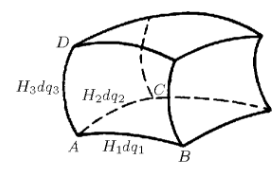
\includegraphics{img/graph}}
\end{figure}

Рассмотрим элемент объема в новых координатах, ограниченный тремя парами координатных поверхностей. Вдоль ребра $A B$ $q_{2}=$ const, $q_{3}=$ const, вдоль $A D \quad q_{1}=$ const, $q_{2}=$ const, вдоль $A C$ $q_{1}=$ const, $q_{3}=$ const. Направляющие косинусы касательной к ребрам $A B, A C$ и $A D$ пропорциональны соответственно
\[
\frac{\partial \varphi_{1}}{\partial q_{1}}, \quad \frac{\partial \varphi_{2}}{\partial q_{1}}, \quad \frac{\partial \varphi_{3}}{\partial q_{1}} ; \quad \frac{\partial \varphi_{1}}{\partial q_{2}}, \quad \frac{\partial \varphi_{2}}{\partial q_{2}}, \quad \frac{\partial \varphi_{3}}{\partial q_{2}} ; \quad \frac{\partial \varphi_{1}}{\partial q_{3}}, \quad \frac{\partial \varphi_{2}}{\partial q_{3}}, \quad \frac{\partial \varphi_{3}}{\partial q_{3}} .
\]

Условие ортогональности ребер будет иметь вид
\[
\frac{\partial \varphi_{1}}{\partial q_{i}} \frac{\partial \varphi_{1}}{\partial q_{k}}+\frac{\partial \varphi_{2}}{\partial q_{i}} \frac{\partial \varphi_{2}}{\partial q_{k}}+\frac{\partial \varphi_{3}}{\partial q_{i}} \frac{\partial \varphi_{3}}{\partial q_{k}}=0 \quad(i \neq k) .
\]

Вычислим элемент длины в новых координатах:
\[
\begin{aligned} 
	d s^{2}=d x^{2}+d y^{2}+ d z^{2}=\left(\frac{\partial \varphi_{1}}{\partial q_{1}} d q_{1}+\frac{\partial \varphi_{1}}{\partial q_{2}} d q_{2}+\frac{\partial \varphi_{1}}{\partial q_{3}} d q_{3}\right)^{2}+ \\
	+\left(\frac{\partial \varphi_{2}}{\partial q_{1}} d q_{1}+\frac{\partial \varphi_{2}}{\partial q_{2}} d q_{2}+\frac{\partial \varphi_{2}}{\partial q_{3}} d q_{3}\right)^{2}+ \\
	+\left(\frac{\partial \varphi_{3}}{\partial q_{1}} d q_{1}+\frac{\partial \varphi_{3}}{\partial q_{2}} d q_{2}+\frac{\partial \varphi_{3}}{\partial q_{3}} d q_{3}\right)^{2} .
\end{aligned}
\]

Раскрывая скобки и учитывая условия ортогональности, получаем
\[
d s^{2}=H_{1}^{2} d q_{1}^{2}+H_{2}^{2} d q_{2}^{2}+H_{3}^{2} d q_{3}^{2},
\]

где
\[
\left.\begin{aligned}
	H_{1}^{2}=\left(\frac{\partial \varphi_{1}}{\partial q_{1}}\right)^{2}+\left(\frac{\partial \varphi_{2}}{\partial q_{1}}\right)^{2}+\left(\frac{\partial \varphi_{3}}{\partial q_{1}}\right)^{2}, \\
	H_{2}^{2}=\left(\frac{\partial \varphi_{1}}{\partial q_{2}}\right)^{2}+\left(\frac{\partial \varphi_{2}}{\partial q_{2}}\right)^{2}+\left(\frac{\partial \varphi_{3}}{\partial q_{2}}\right)^{2}, \\
	H_{3}^{2}=\left(\frac{\partial \varphi_{1}}{\partial q_{3}}\right)^{2}+\left(\frac{\partial \varphi_{2}}{\partial q_{3}}\right)^{2}+\left(\frac{\partial \varphi_{3}}{\partial q_{3}}\right)^{2} \cdot
\end{aligned}\right\}
\]

Вдоль каждого из ребер элементарного объема меняется только одна координата, поэтому для длины этих ребер согласно формуле над системой будем иметь
\[
d s_{1}=H_{1} d q_{1}, \quad d s_{2}=H_{2} d q_{2}, \quad d s_{3}=H_{3} d q_{3},
\]

так что элемент объема равен
\[
d v=d s_{1} d s_{2} d s_{3}=H_{1} H_{2} H_{3} d q_{1} d q_{2} d q_{3} .
\]

Рассмотрим теперь некоторое векторное поле $\mathbf{A}(x, y, z)$. Вычислим $\operatorname{div} \mathbf{A}$, определяемую известной формулой векторного анализа
\[
\operatorname{div} \mathbf{A}=\lim _{v_{M} \rightarrow 0} \frac{\iint_{S} A_{n} d S}{v_{M}},
\]

где $S$ - поверхность, ограничивающая некоторый объем $v_{M}$, содержащий рассматриваемую точку $M$. Применим эту формулу к элементу объема $d v$, изображенному на рисунке.

Пользуясь теоремой о среднем, можно представить разность потоков вектора $\mathbf{A}$ через противоположные грани, например через правую и левую, в виде
\[
Q_{1}=\left.A_{1} d s_{2} d s_{3}\right|_{q_{1}+d q_{1}}-\left.A_{1} d s_{2} d s_{3}\right|_{q_{1}} .
\]

Принимая во внимание формулы для $ds_1, ds_2$ и $ds_3$, получим
\[
\begin{aligned}
	Q_{1}=\left[\left.H_{2} H_{3} A_{1}\right|_{q_{1}+d q_{1}}-\left.H_{2} H_{3} A_{1}\right|_{q_{1}}\right] d q_{2} d q_{3}= \\
	=\frac{\partial}{\partial q_{1}}\left(H_{2} H_{3} A_{1}\right) d q_{1} d q_{2} d q_{3} .
\end{aligned}
\]

Аналогично вычисляются две другие разности потоков через противоположные грани:
\[
\begin{aligned}
	Q_{2} & =\frac{\partial}{\partial q_{2}}\left(H_{3} H_{1} A_{2}\right) d q_{1} d q_{2} d q_{3}, \\
	Q_{3} & =\frac{\partial}{\partial q_{3}}\left(H_{1} H_{2} A_{3}\right) d q_{1} d q_{2} d q_{3} .
\end{aligned}
\]

Подставляя в формулу $\operatorname{div} \mathbf{A}$ значение $\iint_{S} A_{n} d S=Q_{1}+Q_{2}+Q_{3}$ и пользуясь формулой $dv$, получаем выражение дивергенции в криволинейных ортогональных координатах:
\[
\operatorname{div} \mathbf{A}=\frac{1}{H_{1} H_{2} H_{3}}\left[\frac{\partial}{\partial q_{1}}\left(H_{2} H_{3} A_{1}\right)+\frac{\partial}{\partial q_{2}}\left(H_{3} H_{1} A_{2}\right)+\frac{\partial}{\partial q_{3}}\left(H_{1} H_{2} A_{3}\right)\right] .
\]

Предположим, что поле А потенциальное, т. е.
\[
\mathbf{A}=\operatorname{grad} u .
\]

Тогда
\[
A_{1}=\frac{\partial u}{\partial s_{1}}=\frac{1}{H_{1}} \frac{\partial u}{\partial q_{1}} ; \quad A_{2}=\frac{1}{H_{2}} \frac{\partial u}{\partial q_{2}} ; \quad A_{3}=\frac{1}{H_{3}} \frac{\partial u}{\partial q_{3}} .
\]

Подставив в полученную чуть выше формулу для $\operatorname{div} \mathbf{A}$ выражения для $A_{1}, A_{2}, A_{3}$, получим выражение для оператора Лапласа:
\[
\begin{aligned}
	\Delta u=\operatorname{div} \operatorname{grad} u= & \frac{1}{H_{1} H_{2} H_{3}}\left[\frac{\partial}{\partial q_{1}}\left(\frac{H_{2} H_{3}}{H_{1}} \frac{\partial u}{\partial q_{1}}\right)+\right. \\
	& \left.+\frac{\partial}{\partial q_{2}}\left(\frac{H_{3} H_{1}}{H_{2}} \frac{\partial u}{\partial q_{2}}\right)+\frac{\partial}{\partial q_{3}}\left(\frac{H_{1} H_{2}}{H_{3}} \frac{\partial u}{\partial q_{3}}\right)\right] .
\end{aligned}
\]

Таким образом, уравнение Лапласа $\Delta u=0$ в ортогональных криволинейных координатах $q_{1}, q_{2}$ и $q_{3}$ записывается следующим образом:
\[
\begin{aligned}
	\frac{1}{H_{1} H_{2} H_{3}}\left[\frac{\partial}{\partial q_{1}}\right. & \left(\frac{H_{2} H_{3}}{H_{1}} \frac{\partial u}{\partial q_{1}}\right)+ \\
	& \left.+\frac{\partial}{\partial q_{2}}\left(\frac{H_{3} H_{1}}{H_{2}} \frac{\partial u}{\partial q_{2}}\right)+\frac{\partial}{\partial q_{3}}\left(\frac{H_{1} H_{2}}{H_{3}} \frac{\partial u}{\partial q_{3}}\right)\right]=0 .
\end{aligned}
\]

Рассмотрим два частных случая.

\textbf{Сферические координаты.} В этом случае $q_{1}=r, q_{2}=\theta$, $q_{3}=\varphi$ и формулы преобразования принимают вид
\[
x=r \sin \theta \cos \varphi, \quad y=r \sin \theta \sin \varphi, \quad z=r \cos \theta .
\]

Вычислим $d s^{2}$ :
\[
\begin{aligned}
	d s^{2}=(\sin \theta \cos \varphi d r+r \cos \theta \cos \varphi d \theta-r \sin \theta \sin \varphi d \varphi)^{2}+ \\
	\quad+(\sin \theta \sin \varphi d r+r \cos \theta \sin \varphi d \theta+r \sin \theta \cos \varphi d \varphi)^{2}+ \\
	\quad+(\cos \theta d r-r \sin \theta d \theta)^{2} ;
\end{aligned}
\]
после раскрытия скобок и упрощений находим
\[
d s^{2}=d r^{2}+r^{2} d \theta^{2}+r^{2} \sin ^{2} \theta d \varphi^{2},
\]
т. e.
\[
H_{1}=1, \quad H_{2}=r, \quad H_{3}=r \sin \theta .
\]

Подставив значения $H_{1}, H_{2}, H_{3}$ в формулу уравнения Лапласа, получим уравнение Лапласа в сферических координатах:
\[
\frac{1}{r^{2} \sin \theta}\left[\frac{\partial}{\partial r}\left(r^{2} \sin \theta \frac{\partial u}{\partial r}\right)+\frac{\partial}{\partial \theta}\left(\sin \theta \frac{\partial u}{\partial \theta}\right)+\frac{\partial}{\partial \varphi}\left(\frac{1}{\sin \theta} \frac{\partial u}{\partial \varphi}\right)\right]=0,
\]

или окончательно
\[
\Delta_{r, \theta, \varphi} u=\frac{1}{r^{2}} \frac{\partial}{\partial r}\left(r^{2} \frac{\partial u}{\partial r}\right)+\frac{1}{r^{2} \sin \theta} \frac{\partial}{\partial \theta}\left(\sin \theta \frac{\partial u}{\partial \theta}\right)+\frac{1}{r^{2} \sin ^{2} \theta} \frac{\partial^{2} u}{\partial \varphi^{2}}=0 .
\]

\textbf{Цилиндрические координаты.} В этом случае $q_{1}=\rho$, $q_{2}=\varphi, q_{3}=z$ и
\[
x=\rho \cos \varphi, \quad y=\rho \sin \varphi, \quad z=z,
\]

так что
\[
H_{1}=1, \quad H_{2}=\rho, \quad H_{3}=1 .
\]

Уравнение Лапласа в цилиндрических координатах принимает вид
\[
\Delta_{\rho, \varphi, z} u=\frac{1}{\rho} \frac{\partial}{\partial \rho}\left(\rho \frac{\partial u}{\partial \rho}\right)+\frac{1}{\rho^{2}} \frac{\partial^{2} u}{\partial \varphi^{2}}+\frac{\partial^{2} u}{\partial z^{2}}=0 .
\]

Если искомая функция $u$ не зависит от $z$, то уравнение упрощается:
\[
\Delta_{\rho, \varphi} u=\frac{1}{\rho} \frac{\partial}{\partial \rho}\left(\rho \frac{\partial u}{\partial \rho}\right)+\frac{1}{\rho^{2}} \frac{\partial^{2} u}{\partial \varphi^{2}}=0
\] \newpage
	\subsection{Собственные значения и собственные функции задачи Штурма -- Лиувилля
в прямоугольнике. Краевые задачи для уравнений Лапласа и Пуассона в
прямоугольнике}
\subsubsection{Штурм -- Лиувилль}
%ref: Свешников, стр. 56
\label{sec:S-L}
\paragraph{Отрезок.} Рассмотрим следующую \emph{задачу Штурма -- Лиувилля}: 
\[
  \begin{cases}
    \left( k(x) y' \right)' - q(x)y + \lambda\rho(x) y =0, &
    0<x<l,\\
    \left.\alpha_1 y' - \beta_1 y \right|_{x=0} = 0,\\
      \left. \alpha_2 y'+ \beta_2 y \right|_{x=l} = 0.
  \end{cases}
\]
Главное [линейное однородное] уравнение можно переписать в виде $ Ly +\lambda\rho y = 0 $.
Найдём ФСР $ \{y_1(x; \lambda), y_2(x; \lambda)\} $ этого уравнения. Общее
решение тогда будет иметь вид $ y(x) = C_1y_1 + C_2y_2 $, после подстановки в
граничные условия оно образует однородное СЛАУ относительно неизвестных $ C_1 $, $ C_2 $.
Критерий существования ненулевого решения этой системы известен из линейной
алгебры: 
\[
  \left| \begin{matrix}
    \alpha_1y_1'(0;\lambda) - \beta_1y_1(0; \lambda) & \alpha_1y'_2(0;\lambda) -
    \beta_1y_2(0;\lambda) \\
    \alpha_2y'_1(l; \lambda) + \beta_2y_1(l;\lambda) & \alpha_2y'_2(l;\lambda) +
    \beta_2y_2(l;\lambda)
  \end{matrix} \right| = 0.
\]
Этот критерий используется для определения собстенных значений $ \lambda $.
После этого из СЛАУ можно найти\footnote{С точностью до общего множителя, конечно,
который можно найти, если требуется нормировка функций.} соответствующие пары $ (C_1, C_2) $, тем самым
завершив решение задачи.

В ряде случаев алгоритм можно упростить. Например, если найти такую ФСР, что
граничное условие в нуле для $ y_1 $ выполняется, а для $ y_2 $ --- нет, то
после подстановки в первое граничное условие заключаем, что $ C_2 = 0 $, то есть
$ y = C_1y_1 $. Уравнение для $ \lambda $ тогда примет вид  
\[
    \alpha_2 y_1'(l; \lambda) + \beta_2 y_1(l,\lambda) = 0.
\]

\label{sec:prost_sl}
\textbf{Простейший случай}: $ Ly = y'' $, $ \rho \equiv 1 $ с ФСР $
\{\cos\sqrt\lambda x, \sin\sqrt\lambda x\} $ при $ \lambda > 0 $; $ \{x, 1\} $
при $ \lambda = 0 $ и $ \{\ch\sqrt{-\lambda}x, \sh\sqrt{-\lambda}x\} $ при $
\lambda < 0 $.

%TODO: частные случаи или пример (?) (см. там же далее)
%TODO: свойства СЗ и СФ (?) (в приложение?)


\paragraph{Прямоугольник.}
Следующая задача \emph{Лапласа на собственные значения в прямоугольнике},  
\begin{gather*}
    \Delta u + \lambda u = 0, \quad 0 < x < a, \, 0 < y < b,\\
    \left.\alpha_1u_x - \beta_1u\right|_{x=0} = 0, \quad \left.\alpha_2u_x +
      \beta_2u\right|_{x=a} = 0,\\
      \left.\alpha_3 u_y - \beta_3u\right|_{y=0} = 0, \quad \left.\alpha_4u_y +
        \beta_4 u\right|_{y=b} = 0,
\end{gather*}
решается методом разделения переменных: $ u(x, y) = X(x)Y(y) $. После
подстановки и деления на $ XY $ получим 
\[
    \frac{X''}{X} = - \frac{Y''}{Y} - \lambda = -\mu.
\]
Задача распалась на две одномерные задачи Штурма -- Лиувилля: 
\[
  \begin{cases}
    X'' + \mu X = 0, \quad 0 < x < a,\\
    \alpha_1 X'(0) - \beta_1 X(0) = 0,\\
    \alpha_2 X'(a) + \beta_2 X(a) = 0;
  \end{cases} \qquad
  \begin{cases}
    Y'' + \nu Y = 0, \quad 0 < y < b,\\
    \alpha_3 Y'(0) - \beta_3 Y(0) = 0,\\
    \alpha_4 Y'(b) + \beta_4 Y(b) = 0,
  \end{cases}
\]
где $ \nu := \lambda - \mu $.

\subsubsection{Лаплас и Пуассон}
%ref: Пикулин, стр. 28; https://de.ifmo.ru/--books/0051/3/3_4/34yrlappram_1.htm
В уравнении Лапласа $ \Delta u = 0 $ с некоторыми граничными условиями
аналогично разделяем переменные и приходим к соотношению\footnote{Как правило,
  при решении нас не интересует случай $ X''/X < 0 $, однако для большей
  общности можно заменить $
\lambda^2 $ на $ \lambda $.}
\[
  \frac{X''}{X} = - \frac{Y''}{Y} =: \lambda^2,  
\]
которое порождает две одномерные задачи Штурма -- Лиувилля с соответствующими
граничными условиями. При этом первая из них --- $ Y'' + \lambda^2Y = 0 $ --- с
тригонометрической ФСР\footnote{См. выше <<простейший
случай>>.}, а вторая --- $ X'' - \lambda^2X = 0 $ --- с гиперболической
(конечно, может интересовать и линейный случай $ \lambda = 0 $).

В уравнении Пуассона $ \Delta u = f(x, y) $ с некоторыми граничными условиями
аналогично разделяем переменные и приходим к вспомогательной однородной задаче
$ X'' + \lambda^2 X = 0 $. Собственные функции $ X_n(x) $ этой задачи образуют
полную ортогональную систему, поэтому можем представить решение в виде $ u(x,
y)= \sum Y_n(y) X_n(x) $, где осталось найти лишь $ Y_n(y) $. Подставим эту
форму решения, параллельно разложив\footnote{Координата есть отношение проекции
$ (f, X_n)/\|X_n\| $ к длине.}
\begin{equation}
  \label{eq:razl}
  f_n(y) = \frac{1}{\|X_n\|^2} \int\limits_{0}^{a}
  f(x, y) X_n(x)\,dx
\end{equation}
неоднородную часть $ f(x, y) $ по базису $ X_n(x) $. Получим  
\[
  \sum_{n=0}^\infty X_n''(x)Y_n(y) + \sum_{n=0}^\infty X_n(x)Y_n''(y) =
  \sum_{n=0}^\infty f_n(y)X_n(x),
\]
откуда получаем бесконечность уравнений на $ Y_n(y) $ (с соответствующими граничными условиями)
\[
  \frac{X''_n}{X_n} Y_n + Y_n'' = f_n.
\]
Решая это НЛДУ в общем виде, получаем ответ.


 \newpage
	\subsection{Метод разделения переменных решения первой краевой задачи для уравнения Лапласа внутри круга и вне круга. Интеграл Пуассона}
%aut: Slava
\subsubsection{Лаплас}
\label{sec:16}
%ref: С-Т, стр. 328 (основное); Пикулин, стр. 18
Рассмотрим уравнение Лапласа $ \Delta u = 0 $ внутри круга радиуса $ \rho $ с граничным условием
$ u(\rho, \varphi) = f(\varphi) $. Некоторые дополнительные условия: $ u $ непрерывна внутри круга, $ f
$ непрерывно дифференцируема. От условия на $ f $ можно избавиться.

Перейдём в полярные координаты с центром в центре круга. Там\footnote{См. раздел
\ref{sec:14}.}
\[
    \Delta u = \frac{1}{r} \frac{\partial}{\partial r}\left( r \frac{\partial
    u}{\partial r} \right) + \frac{1}{r^2}\frac{\partial^2 u}{\partial
  \varphi^2} = 0.
\]
Разделим переменные и после подстановки получим
\[
    \frac{(rR')'}{R/r} = - \frac{\Phi''}{\Phi} = \lambda \geqslant 0.
\]
Соответствующая задача Штурма -- Лиувилля $ \Phi'' + \lambda\Phi = 0 $
тогда будет иметь тригонометрические решения\footnote{См. раздел \ref{sec:prost_sl}, <<простейший
случай>>.} $ \Phi = A\cos\sqrt\lambda \varphi + B\sin\sqrt\lambda \varphi $.
При этом условия начальной системы функции $ \Phi $ не касаются, однако из
однозначности решения вытекает $ 2\pi $-периодичность функции $ \Phi(\varphi)
$\footnote{Отсюда и требование к знаку $ \lambda $. Заметим, что случай
$ \lambda = 0 $, $\Phi \equiv \mathrm{const} = A $ входит в обозрение.}.
Это условие можно записать официально как\footnote{Говорить о периодичности
  здесь не совсем корректно, поскольку и так $ \varphi \in [0, 2\pi) $.
Требуется лишь, чтобы для любого $ n $ $ \Phi^{(n)}(0) = \Phi^{(n)}(2\pi) $.
Тогда после возвращения в декартовы координаты функция $ u $ будет непрерывной
со всеми своими производными.} $ \Phi(0) = \Phi(2\pi) $, $ \Phi'(0) =
\Phi'(2\pi) $. Из самого уравнения вытекает тогда, что $ \Phi^{(n)}(0) =
\Phi^{(n)}(2\pi) $ для любого $ n $. После подстановки $ \Phi $ в условия спектр
быстро угадывается, однако можно и строго прийти к уравнению\footnote{См. раздел
\ref{sec:S-L}.} 
\[
  \left(\cos ( \sqrt\lambda 2\pi ) - 1\right)^2 + \sin^2 \left(\sqrt\lambda2\pi\right)=0,
\]
откуда уже явно видно, что $ \lambda_n = n^2 $.

Функцию $ R(r) $, как решение уравнения Эйлера, будем искать в виде $ R(r) = r^\mu $.
Подставляя и сокращая, получаем $ n^2 = \mu^2 $, а $ R(r) = Cr^n + Dr^{-n} +
E\ln r + F$.
Теперь, исходя из ограниченности гармонических функций и условий задачи, приравниваем один из
коэффициентов $ C $, $ D $, а также коэффициент $ E $ к нулю и получаем частные
решения
\begin{align*}
  u_n(r,\varphi) &= r^n(A_n\cos n\varphi + B_n \sin n\varphi) \quad \text{для
  задачи внутри круга},\\
    u_n(r,\varphi) &= r^{-n}(A_n\cos n\varphi + B_n \sin n\varphi) \quad \text{для
  задачи вне круга}.
\end{align*}
Учитывая получившийся вид решения, разложим граничное условие $ f(\varphi) $ в
ряд Фурье 
\begin{equation}
    \alpha_0 = \frac{1}{\pi}\int\limits_{-\pi}^{\pi}f(\psi)\,d\psi, \quad
    \alpha_n = \frac{1}{\pi}\int\limits_{-\pi}^{\pi}f(\psi)\cos
    n\psi\,d\psi,\quad
    \beta_n = \frac{1}{\pi}\int\limits_{-\pi}^{\pi}f(\psi)\sin n\psi\,d\psi
    \label{eq:fourier_exp}
\end{equation}
и приравняем коэффициенты ряда $ u(a, \varphi) $, откуда уже получим $ A_n $ и $ B_n $.
Конкретно, 
\begin{align}
  f(\varphi) &= \frac{\alpha_0}{2} + \sum_{n=1}^\infty(\alpha_n\cos n\varphi +
  \beta_n \sin n\varphi),\\
  u(\rho, \varphi) &= \frac{\alpha_0}{2} + \sum_{n=1}^\infty t^n (\alpha_n\cos
  n\varphi + \beta_n \sin n\varphi), \label{eq:fourier_sol}
\end{align}
где $ t = r/a \leqslant 1 $ для внутренней задачи и
$ t = a/r \leqslant 1 $ для внешней.

%TODO: как раскладывать в ряд Фурье (?)
%TODO: формулы для An Bn (?)



\subsubsection{Интеграл Пуассона}
%ref: С-Т, стр. 333; Пикулин, стр. 20 (основное); Олейник, стр. 86; Шубин, стр. 130;
%Свешников, стр. 212; Петровский, стр. 251
Ограничимся на время внутренним случаем и соединим формулы
\eqref{eq:fourier_exp} и \eqref{eq:fourier_sol}:
\[
  u(r,\varphi) = \frac{1}{\pi} \int\limits_{-\pi}^{\pi} \left[ \frac{1}{2} + \sum_{n=1}^\infty \left(
  \frac{r}{a} \right)^n (\cos n\psi\cos n\varphi + \sin n\psi \sin n\varphi
)\right] \, d\psi.
\]
Используя формулы косинуса суммы, Эйлера, суммы геометрической прогрессии,
комплексную формулу косинуса, при
$ t := r/a < 1 $ получим
\begin{multline*}
    \frac{1}{2} + \sum t^n(\cos n\psi \cos n\varphi + \sin n\psi \sin n\varphi)
    = \frac{1}{2} + \sum t^n \cos n(\varphi - \psi) =\\=
    \frac{1}{2} + \frac{1}{2}\sum t^n \left[ e^{in(\varphi-\psi)} +
    e^{-in(\varphi - \psi)} \right] = \frac{1}{2} \left( 1 + \sum \left[
(te^{i(\varphi - \psi)})^n + (te^{-i(\varphi - \psi)})^n \right]  \right) =\\=
  \frac{1}{2} \left[ 1 + \frac{te^{i(\varphi - \psi)}}{1 - te^{i(\varphi-\psi)}}
    + \frac{te^{-i(\varphi - \psi)}}{1 - te^{-i(\varphi-\psi)}}\right] =
    \frac{1}{2} \frac{1 - t^2}{1 - 2t\cos(\varphi - \psi) + t^2}.
\end{multline*}
Таким образом, \emph{интегралом Пуассона} называется интеграл 
\[
    \frac{1}{2\pi} \int\limits_{-\pi}^{\pi}f(\psi) K(r, \varphi, a,
    \psi)\,d\psi,
\]
а выражение  
\[
    K(r,\varphi, a,\psi) = \frac{a^2 - r^2}{r^2 - 2ar\cos(\varpsi-\psi) + a^2}
\]
называют \emph{ядром Пуассона}. Видно, что $ K > 0 $, поскольку при $ r < a $ и
$ 2ar < a^2 + r^2 $. При $ r = a $ интеграл теряет смысл, однако в пределе при
$ r \to a $ стремится\footnote{Поскольку ряд, из
которого был получен интеграл, непрерывен в замкнутой области.} к граничной функции $ f(\varphi) $, что позволяет
доопределить его соответствующим образом и назвать решением $
u(r,\varphi) $.

Понятно, что для внешней задачи надо просто
поменять числитель ядра на $ r^2 - a^2 $.

%Интеграл Пуассона в комплексной записи (см., например, Пикулин)
 \newpage
	\subsection{Функция Грина уравнения Лапласа первой краевой задачи в круге, на полуплоскости в полупространстве. Метод отражений.}
%autor: Сеня, Слава (первый раздел)
\subsubsection{Введение. Основная формула Грина}
\paragraph{Случай $ \mathbb R^3 $.}
Ранее была получена \emph{вторая формула Грина} \eqref{eq:green2}. Легко
заметить\footnote{Надо записать уравнение Лапласа в сферических координатах, где
функцию $ v $ считать зависимой только от $ r $ и проинтегрировать ОДУ.}, что
функция $ v(M) = 1/R_{MM_0} $ является гармонической\footnote{То есть
  удовлетворяет уравнению Лаплама. Символом $ R_{MM_0} $ обозначается расстояние
$ MM_0 $.} при $ M \neq M_0 $. Подставим эту функцию во вторую формулу Грина для
некоторой области $ T\setminus U(M_0; \varepsilon) $\footnote{Обозначения: $ U(M_0;
\varepsilon) $ --- шар с центром в особой точке $ M_0 $ и радиусом $ \varepsilon
$; $ \partial U(M_0; \varepsilon) $ --- его граница.}, где нет особых точек: 
\[
  \iiint\limits_{T\setminus U} \left( u\Delta \frac{1}{R} - \frac{1}{R}\Delta u \right)
  dxdydz = \iint\limits_{\partial T} \left( u \frac{\partial}{\partial n}
  \left(\frac{1}{R}\right) - \frac{1}{R} \frac{\partial u}{\partial n} \right)
  \,d\sigma + \iint\limits_{\partial U} u \frac{\partial}{\partial n} \left(
  \frac{1}{R} \right) \, d\sigma - \iint\limits_{\partial U} \frac{1}{R}
  \frac{\partial u}{\partial n}\,d\sigma.
\]
Теперь заметим, что 
\begin{align*}
  \frac{\partial}{\partial n} \left( \frac{1}{R} \right) \bigg|_{\partial U} &= -
  \frac{\partial}{\partial r} \left( \frac{1}{R} \right) \bigg|_{r=\varepsilon} =
  \frac{1}{\varepsilon^2},\\
  \iint\limits_{\partial U} u \frac{\partial}{\partial n} \left( \frac{1}{R}
\right)\, d\sigma &= \frac{1}{\varepsilon^2} 4\pi\varepsilon^2 u^\ast = 4\pi
  u^\ast,
\end{align*}
где $ u^\ast $ --- среднее значение функции $ u(M)|_{\partial U} $. Аналогично 
\[
  \iint\limits_{\partial U} \frac{1}{R} \frac{\partial u}{\partial n}\,d\sigma =
  \frac{1}{\varepsilon} 4\pi\varepsilon^2 \left( \frac{\partial u}{\partial n}
  \right)^\ast = 4\pi\varepsilon \left( \frac{\partial u}{\partial n}
  \right)^\ast.
\]
Заметим также, что при $ \varepsilon \to 0 $ верно $ u^\ast \to u(M_0) $ и $
4\pi\varepsilon (\partial u/\partial n)^\ast \to 0 $. Так мы пришли к
\emph{основной интегральной формуле Грина} 
\begin{equation}\label{eq:green3}
  4\pi u(M_0) = - \iint\limits_{\partial T} \left[ u(P) \frac{\partial}{\partial
  n} \left( \frac{1}{R_{M_0 P}} \right)  - \frac{1}{R_{M_0 P}}\frac{\partial
u}{\partial n} \right] \,d\sigma - \iiint\limits_T \frac{\Delta
u(M)}{R_{M_0M}}\,dxdydz,
\end{equation}
где $ P $ --- некоторая граничная точка области $ T $. До этого предполагалось,
что $ M_0 \in T $. При $ M_0 \in \partial T$ несложно прийти к формуле
\eqref{eq:green3}, где слева вместо $ 4\pi $ стоит $ 2\pi $ (поскольку там имеем
вместо $ U(M_0; \varepsilon) $ поверхность, чей объём при малых $ \varepsilon $
близок к половине объёма шара). Если $ M_0 $ не
принадлежит замыканию $ T $, то функция $ v $ гармонична во всей области, и
вместо $ 4\pi $ следует поставить ноль.

\paragraph{Случай $ \mathbb R^2 $.}
Совершенно аналогично, только для гармоничности теперь $ v = \ln(1/R) $, тройные
интегралы меняются на двойные\ldots, а в уравнении \eqref{eq:green3} коэффициент
слева теперь принимает значения соответственно в таких же условиях $ 2\pi $, $ \pi $ и 0.

\paragraph{Функция источника.} Попробуем с полученными знаниями решить уравнение $ \Delta u  = 0 $. Пусть функция $ v(M) \in C^1(\bar T) $, $ \Delta v = 0 $ не имеет особенностей.
Согласно второй формуле Грина \eqref{eq:green2} в этом случае 
\[
  0 = \iint\limits_{\partial T} \left( v \frac{\partial u}{\partial n} - u
  \frac{\partial v}{\partial n} \right) \,d\sigma - \iiint\limits_T v\Delta
  u\,dxdydz. 
\]
Сложим теперь это равенство с основной формулой Грина \eqref{eq:green3}  и
получим 
\[
  u(M_0) = \iint\limits_{\partial T} \left( G \frac{\partial u}{\partial n} - u
  \frac{\partial G}{\partial n}\right) \,d\sigma - \iiint\limits_T \Delta u
  \cdot G\,dxdydz,
\]
где 
\begin{equation}\label{eq:green-func}
  G(M, M_0) := \frac{1}{4\pi R_{MM_0}} + v.
\end{equation}
Функция $ v $ по понятным причинам выбирается так, чтобы $ G|_{\partial T} = 0 $ в случае первой
краевой задачи (Дирихле) и $ \partial G/\partial n |_{\partial T} = 0 $ для
второй (Неймана). Определим $ G $ с помощью следующих условий:
\begin{enumerate}
  \item $G(M, P)$ как функция точки $ P $ гармоническая всюду при $ P \neq M $.
  \item $ G(M, P = M) $ равна бесконечонсти и представима в виде
    \eqref{eq:green-func}, где $ \Delta v = 0 $ всюду в $ T $.
  \item $ G(M, P)|_{P\in\partial T} = 0 $. Для этого положим $ v|_{\partial T} =
    -1/(4\pi R)$.
\end{enumerate}
Таким образом, например, решение задачи Дирихле с граничной функцией $ f $
уравнения Лапласа есть 
\[
  u(M_0) = - \iint\limits_{\partial T} f \frac{\partial G}{\partial n}\,d\sigma.
\]

Двумерная функция источника строится с аналогичными условиями и имеет вид 
\[
  G = \frac{1}{2\pi} \ln \frac{1}{R_{MM_0}} + v(M, M_0), \quad \Delta v = 0, \
  v|_{\partial T} = - \frac{1}{2\pi} \ln \frac{1}{R}.
\]



\paragraph{Метод отражений (метод электростатических изображений).}\footnote{Т.-С. стр. 343}

%TODO: мотивация
Для построения функции источника в виде
\begin{equation*}
	G(M, M_0) = \frac{1}{4 \pi R_{M M_0}} + v
\end{equation*}
индуцированное поле $v$ представляется как поле зарядов, расположенных вне поверхности $\Sigma$ и выбираемых таким образом, чтобы выполнялось условие
\begin{equation*}
	v|_{\Sigma} = -\frac{1}{4 \pi R}.
\end{equation*}

Приведем примеры построения функции источника методом отражений.
Пусть дана сфера радиуса $R$ с центром в точке $O$.
Поместим в точку $M_0$ единичный заряд и отложим на радиусе, проходящем через точку $M_0$, такой отрезок $OM_1$, что
\begin{equation} \label{section}
	\rho_0 \rho_1 = R^2,
\end{equation}
где $\rho_0 = \abs{OM_0}$ и $\rho_1 = \abs{OM_1}$. 

\begin{figure}[H]
	\centering
	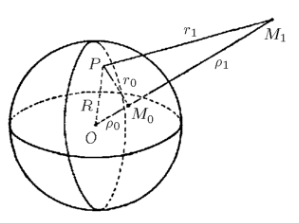
\includegraphics[width=0.4\linewidth]{img/sphere_green}
	\caption{}
\end{figure}

Точки $M_0$ и $M_1$ называются сопряженными друг другу. 

Докажем, что для всех точек $P$ на сфере, расстояния до $M_0$ и $M_1$ пропорциональны. Рассмотрим $\triangle OPM_0$ и $\triangle OMP_1$. Они подобны по общему углу и двум пропорциональным сторонам
\begin{equation*}
	\frac{\rho_0}{R} = \frac{R}{\rho_1}, \text{ или } \frac{\abs{OM_0}}{R} = \frac{R}{\abs{OM_1}}.
\end{equation*}
Из подобия следует
\begin{equation} \label{prop}
	\frac{r_0}{r_1} = \frac{\rho_0}{R} = \frac{R}{\rho_1},
\end{equation}
где $r_0 = \abs{\overrightarrow{M_0P}}$, $r_1 = \abs{\overrightarrow{M_1 P}}$. Из пропорции \eqref{prop} получаем  
\begin{equation*}
	r_0 = \frac{\rho_0}{R} r_1
\end{equation*}
для всех точек сферы. Поэтому гармоническая функция $v = -R/\rho_0 \cdot 1/r_1$ на сфере принимает то же значение, что и функция $-1/r_0$. она представляет, очевидно потенциал заряда величины $-R/\rho_0$, помещенного в точку $M_1$.

Таким образом 
\begin{equation} \label{final_green}
	G(P, M_0) = \frac{1}{4 \pi} \Bigg(\frac{1}{r_0} - \frac{R}{\rho_0} \frac{1}{r_1}\Bigg)
\end{equation}

\paragraph{Функция источника для круга.}\footnote{Т.-С. стр. 346}

Функция источника для круга может быть получена таким же способом, как и функция источника для сферы. В этом случа ее следует искать в виде
\begin{equation}
	G = \frac{1}{2 \pi} \ln{\frac{1}{r}} + v.
\end{equation}

Повторяя рассуждения от \eqref{section} до \eqref{final_green}, мы найдем функцию $G$ в виде 
\begin{equation}
	G = \frac{1}{2 \pi} \Bigg[\ln{\frac{1}{r_0}} - \ln{\frac{R}{\rho_0} \frac{1}{r_1}}\Bigg],
\end{equation}
где $\rho_0 = \abs{OM_0}$, $r_0 = \abs{M_0 P}$, $r_1 = \abs{M_1 P}$, $R = \abs{OP}$ --- радиус круга (см. рис. \ref{circle_green}).
\begin{figure}[H]
	\centering
	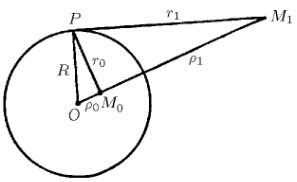
\includegraphics[width=0.4\linewidth]{img/circle_green}
	\caption{}
	\label{circle_green}
\end{figure}
Нетрудно убедиться в том, что определенная таким образом гармоническая функция обращается в нуль на границе: $G|_{C} = 0$.

\paragraph{Функция источника для полупространства.}\footnote{Т.-С. стр. 347}

Найдем функцию источника для полупространства $z > 0$. Поместим в точку $M_0(x_0, y_0, x_0)$ единичный заряд, который создает в неограниченном пространстве поле, потенциал которого определяется функцией 
\begin{equation*}
	\frac{1}{4 \pi} \frac{1}{R_{M_0 M}}, \text{ где } R_{M_0 M} = \sqrt{(x - x_0)^2 + (y - y_0)^2 + (z - z_0)^2}.
\end{equation*}
Нетрудно видеть, что "индуцированное поле" $v$ является полем отрицательного единичного заряда, помещенного в точку $M_1(x_0, y_0, -z_0)$, являющуюся зеркальным изображением точки $M_0$ в плоскости $z = 0$ (рис. \ref{halfdim_green}). 
Функция $G$, равная
\begin{equation*}
	G(M, M_0) = \frac{1}{4 \pi R_0} - \frac{1}{4 \pi R_1},
\end{equation*}
где
\begin{align*}
	R_0 = \abs{\overrightarrow{M_0 M}} = \sqrt{(x - x_0)^2 + (y - y_0)^2 + (z - z_0)^2}, \\
	R_1 = \abs{\overrightarrow{M_1 M}} = \sqrt{(x - x_0)^2 + (y - y_0)^2 + (z - z_0)^2}, \\
\end{align*}
обращается в нуль при $z = 0$ и имеет нужную особенность в точке $M_0$.

\begin{figure}[H]
	\centering
	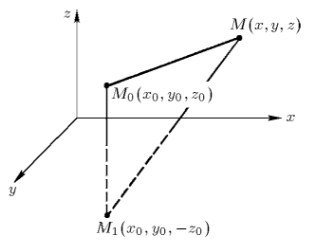
\includegraphics[width=0.4\linewidth]{img/halfdim_green}
	\caption{}
	\label{halfdim_green}
\end{figure}
 \newpage
	\subsection{Единственность решения краевой задачи (внутренней и внешней) для уравнения Лапласа.}

При исследовании стационарных процессов различной физической природы (колебания, теплопроводность, диффузия и др.) обычно приходят к уравнениям эллиптического типа. Наиболее распространенным уравнением этого типа является уравнение Лапласа
\begin{equation*}
	\Delta u = 0. 
\end{equation*}

Функция $u$ называется гармонической в области $T$, если она непрерывна в этой области вместе со своими производными до 2-го порядка и удовлетворяет уравнению Лапласа. 

Рассмотрим некоторый объем $T$, ограниченный поверхностью $\Sigma$.
Краевые задачи формулируются следующим образом.

\textit{Найти функцию $u(x, y, z)$, удовлетворяющую внутри $T$ уравнению Лапласа и граничному условию, которое может быть взято в одном из следующих видов:} 
\begin{enumerate}
	\item $u = f_1 $ на $ \Sigma $ \quad \quad \quad \quad \quad \quad \quad \quad \texttt{(первая краевая задача)},
	
	\item $\frac{\partial u}{\partial n} = f_2$ на $ \Sigma $ \quad \quad \quad \quad \quad \quad \quad \texttt{(вторая краевая задача)},
	
	\item $\frac{\partial u}{\partial n} + h(u - f_3) = 0$ на $ \Sigma $ \quad \quad \texttt{(третья краевая задача)},
\end{enumerate}
\textit{где $f_1, f_2, f_3, h$ --- заданные функции, $\partial u / \partial n$ --- производная по внешней нормали к поверхности $\Sigma$}.

Первую краевую задачу для уравнения Лапласа часто называют задачей Дирихле, вторую --- задачей Неймана.

Если ищется решение в области $T_0$, внутренней (или внешней) по отношению к поверхности $\Sigma$, то соответствующую задачу называют внутренней (или внешней) краевой задачей. 

\textit{Первая внутренняя краевая задача для уравнения Лапласа не может иметь двух различных решений}.

Допустим, что существуют две различные функции $u_1$ и $u_2$, являющиеся решениями задачи, т.е. функции, непрерывные в замкнутой области $T + \Sigma$, удовлетворяющие внутри области уравнению Лапласа и на поверхности $\Sigma$ принимающие одни и те же значения $f$. Разность этих функций $u = u_1 - u_2$ обладает следующими свойствами:
\begin{enumerate}
	\item $\Delta u = 0$ внутри области $T$;
	
	\item $u$ непрерывна в замкнутой области $T + \Sigma$;
	
	\item $u|_{\Sigma} = 0.$
\end{enumerate}

Функцию $u(M)$, таким образом, непрерывна и гармонична в области $T$ и равна нулю на границе. Как известно, всякая непрерывная функция в замкнутой области достигает своего максимального значения (п. \ref{maximum_principle}). Убедимся в том, что $u \equiv 0$. Если функция $u \not \equiv 0$ и хотя бы в одной точке $u > 0$, то она должна достигать положительного максимального значения внутри области, что невозможно. Совершенно так же доказывается, что функция $u$ не может принимать внутри $T$ отрицательных значений. Отсюда следует, что 
\begin{equation*}
	u \equiv 0.
\end{equation*}

Согласно следствию из принципа максимума, если функция $u$ гармоническая вне области $G$, и $u(\infty) = 0$, то так же можно говорить, что 
\begin{equation*}
	\abs{u(x)} \leqslant \max\limits_{\xi \in S}{\abs{u(\xi)}}, \quad x \in \bar{G_1}, G_1 = \mathbb{R}^n \ \bar{G}  
\end{equation*}

Поэтому единственность доказывается аналогично внутреннему случаю. 

\textit{Докажем, что решение второй внутренней краевой задачи определяется с точностью до произвольной постоянной.}

Доказательство проведем при дополнительном предположении, что функция $u$ имеет непрерывные первые производные в области $T + \Sigma$. 

Пусть $u_1$ и $u_2$ --- две непрерывно дифференцируемые в $T + \Sigma$ функции, удовлетворяющие уравнению $\Delta u = 0$ в $T$ и условию $\partial u/ \partial n |_{\Sigma} = f(M)$ на $\Sigma$. Для функции $u = u_1 - u_2$ будем иметь 
\begin{equation*}
	\frac{\partial u}{\partial n} \Big|_{\Sigma} = 0.
\end{equation*}
Полагая в первой формуле Грина (...%TODO) $v = u$ и учитывая соотношения $\Delta u = 0$ и $\partial u / \partial n |_{\Sigma} = 0$, получаем 
\begin{equation*}
	 \iiint \limits_{T} \Bigg[\Bigg(\frac{\partial u}{\partial x}\Bigg)^2 + \Bigg(\frac{\partial u}{\partial y}\Bigg)^2 + \Bigg(\frac{\partial u}{\partial z}\Bigg)^2\Bigg] \, d\tau = 0.
\end{equation*}

Отсюда в силу непрерывности функции $u$ и ее первых производных следует 
\begin{equation*}
	\frac{\partial u}{\partial x} = \frac{\partial u}{\partial y} = \frac{\partial u}{\partial z} \equiv 0, \quad \text{ т.е. } u \equiv const,
\end{equation*}
что и требовалось доказать. 

Изложенный метод применим и в случае неограниченной области для функций, удовлетворяющих требованиям регулярности на бесконечности.
\newline 

\textit{Докажем, что внешняя краевая задача имеет единственное решение, регулярное на бесконечности.}

В случае неограниченной области для функции, внешней к замкнутой поверхности формула Грина применима и имеет вид:
\begin{equation} \label{out_green}
	\iiint \limits_{T} u \Delta v \, d\tau = - \iiint \limits_{T} \Bigg[\frac{\partial u}{\partial x}\frac{\partial v}{\partial x} + \frac{\partial u}{\partial y}\frac{\partial v}{\partial y} + \frac{\partial u}{\partial z}\frac{\partial v}{\partial z}\Bigg] \, d\tau + \iint \limits_{\Sigma} u \frac{\partial v}{\partial n} \, d\sigma.
\end{equation}

Полагая в ней $v = u = u_1 - u_2$ и учитывая, что $\Delta u = 0$ и $\partial u / \partial n |_{\Sigma} = 0$, получаем
\begin{equation}
	\iiiint \limits_{T} (u_x^2 + u_y^2 + u_z^2) \, d\tau = 0.
\end{equation}
Отсюда в силу непрерывности производных функции $u$ следует, что 
\begin{equation*}
	u_x = 0, \quad u_y = 0, \quad u_z = 0 \text{ и } u \equiv const. 
\end{equation*}
Так как $u = 0$ на бесконечности, то
\begin{equation}
	u \equiv 0, \text{ т.е. } u_1 \equiv u_2,
\end{equation}
что и требовалось доказать.   \newpage
	\subsection{Первая и вторая формулы Грина в ограниченной области. Потенциалы простого и
двойного слоя. Их свойства, физический смысл.}

\paragraph{Первая формула Грина}

В Тихонове-Самарском (стр. 307) даётся такая первая формула Грина:
\begin{equation} \label{first_green_formula}
	\iiint \limits_T u \Delta v \, d\tau
	= \iint \limits_\Sigma u \dfrac{\partial v}{\partial n} \, d\sigma
	- \iiint \limits_T \left(
	\dfrac{\partial u}{\partial x} \dfrac{\partial v}{\partial x} + 
	\dfrac{\partial u}{\partial y} \dfrac{\partial v}{\partial y} + 
	\dfrac{\partial u}{\partial z} \dfrac{\partial v}{\partial z} \right) \, d\tau,
\end{equation}
где $T$ -- некоторый объём, органиченный поверхностью $\Sigma$;
$u(x, y, z), v(x, y, z)$ -- непрерывно-дифференцируемы внутри $T+\Sigma$;
$\dfrac{\partial}{\partial n} = \cos\alpha \dfrac{\partial}{\partial x} 
  + \cos\beta \dfrac{\partial}{\partial y} 
  + \cos\gamma \dfrac{\partial}{\partial z}$ -- производная по направлению внешней нормали.
Эта формула является прямым следствием формулы Остроградского-Гаусса. Причём можно чуть упростить
запись этой формулы, если вспомнить что такое градиент:
$\grad u = \nabla u = \left( \dfrac{\partial u}{\partial x}, 
  \dfrac{\partial u}{\partial y},
  \dfrac{\partial u}{\partial z} \right) $:
\[
  \iiint \limits_T u \Delta v \, d\tau
  = \iint \limits_\Sigma u \dfrac{\partial v}{\partial n} \, d\sigma
    - \iiint \limits_T \nabla u \cdot \nabla v \, d\tau,
\]

\paragraph{Вторая формула Грина}

Рассматривая разницу первых формул Грина, применённых к $u \Delta v$ и $v \Delta u$, можно
получить вторую формулу Грина:
\[
  \iiint \limits_T \left( u \Delta v - v \Delta u \right) \, d\tau
  = \iint \limits_\Sigma \left( u \dfrac{\partial v}{\partial n} - v \dfrac{\partial u}{\partial n}  \right) \, d\sigma
\]

\paragraph{Потенциалы простого и двойного слоя}

Я не стал переделывать обозначения, поэтому просто: область у нас G, поверхность, которая ее
ограничивает -- $S$, и, если я правильно понял, $G_1 = \mathbb{R}^n \backslash \bar G$. 

Следующая формула в Тихонове-Самарском называется \emph{основной интегральной формулой Грина}
\footnote{Тихонов-Самарский стр 310}, а во Владимирове называется просто формулой Грина
\footnote{Владимиров, стр. 262}.

Пусть $u \in \mathcal{C}^2 (\bar G)$ и $u(x) = 0, x \in G_1$; тогда при $x \notin S$ справедлива
следующая формула Грина (это из Владимирова):
\begin{align*}
  u(x) &= - \dfrac{1}{(n-2) \sigma_n} \int\limits_G \dfrac{\Delta u(y)}{|x-y|^{n-2}} \, dy
  + \dfrac{1}{(n-2) \sigma_n} \int\limits_S \left[ 
    \dfrac{1}{|x-y|^{n-2}} \dfrac{\partial u(y)}{\partial n} 
    - u(y) \dfrac{\partial }{\partial n_y} \dfrac{1}{|x-y|^{n-2}}\right] \, dS_y, n \geqslant 3, \\
  u(x) &= - \dfrac{1}{2\pi} \int\limits_G \Delta u(y) \ln \dfrac{1}{|x-y|} \, dy
  + \dfrac{1}{2\pi} \int\limits_S \left[ 
    \ln \dfrac{1}{|x-y|} \dfrac{\partial u(s)}{\partial n} 
    - u(y) \dfrac{\partial }{\partial n_y} \ln \dfrac{1}{|x-y|} \right] \, dS_y, n=2
\end{align*}
Другими словами, в области $G$ функция $u(x)$ представляется в виде суммы трёх ньютоновых
(логарифмических) потенциалов:
\[
  u(x) = V_n(x) + V_n^{(0)} (x) + V_n^{(1)} (x), x\in G,
\]
где (считаем для определенности $n \geqslant 3$)
\[
  V_n(x) = \mathcal{E}_n * \left\{ \Delta u \right\} = - \dfrac{1}{(n-2) \sigma_n} \int_G \dfrac{\Delta u(y)}{|x-y|^{n-2}} \, dy
\]
-- объёмный потенциал с плотностью $- \dfrac{1}{(n-2) \sigma_n} \left\{ \Delta u \right\}$;

\[
  V_n^{(0)} (x) = - \mathcal{E} * \left( \dfrac{\partial u}{\partial n} \delta_S \right) 
  = \dfrac{1}{(n-2) \sigma_n} \int_S \dfrac{1}{|x-y|^{n-2}} \dfrac{\partial u(y)}{\partial n} \, dS_y
\]
-- потенциал простого слоя на $S$ с поверхностной плотностью $\dfrac{1}{(n-2) \sigma_n} \dfrac{\partial u}{\partial n}$;

\[
  V_n^{(1)} (x) = - \mathcal{E}_n * \dfrac{\partial }{\partial n} (u \delta_S)
  = - \dfrac{1}{(n-2) \sigma_n} \int_S u(y) \dfrac{\partial }{\partial n_y} \dfrac{1}{|x-y|^{n-2}} \, dS_y
\]
-- потенциал двойного слоя на $S$ с поврехностной плотностью $-\dfrac{1}{(n-2) \sigma_n} u$

Формула Грина справедлива и для функций $u$ класса
$\mathcal{C}^2 (G) \bigcap \mathcal{C}^1 (\bar G)$, если в ней интеграл по области $G$ понимать
как несобственный. (Этот интеграл может сходиться не абсолютно.)

Для гармонической в области $G$ функции $u$ класса $\mathcal{C}^1 (\bar G)$ формула Грина принимает
следующий вид:
\begin{align*}
  u(x) &= \dfrac{1}{(n-2) \sigma_n} \int_S \left[ 
    \dfrac{1}{|x-y|^{n-2}} \dfrac{\partial u(y)}{\partial n}
    - u(y) \dfrac{\partial }{\partial n_y} \dfrac{1}{|x-y|^{n-2}}\right] \, dS_y, n \geqslant 3, \\
  u(x) &= \dfrac{1}{2\pi} \int_S \left[ 
    \ln \dfrac{1}{|x-y|} \dfrac{\partial u(y)}{\partial n}
    - u(y) \dfrac{\partial }{\partial n_y} \ln \dfrac{1}{|x-y|}\right] \, dS_y, n=2
\end{align*}

Поверхностные потенциалы $V_n{(0)}$, $V_n^{(1)}$ можно непрерывно дифференцировать вне $S$ под
знаком интеграла бесконечное число раз, и эти потенциалы -- гармонические функции вне $S$.

% TODO дописать физический смысл и свойства
 \newpage
	\subsection{Собственные значения и собственные функции задачи Штурма -- Лиувилля
в круге, в круговом кольце и во внешности круга. Краевые задачи для уравнения
Лапласа в указанных областях}\label{sec:20}
\subsubsection{Штурм -- Лиувилль}
%aut: Slava
%ref: Свешников, стр. 117
Рассматривается задача
\[
  \begin{cases}
    \Delta u + \lambda u = 0,\\
    \alpha u(a, \varphi)_n + \beta u(a, \varphi) = 0.
  \end{cases}
\]
Напомним\footnote{См. раздел \ref{sec:14}.}, что  
\[
    \Delta u = \frac{1}{r} \frac{\partial}{\partial r} \left( r \frac{\partial
    u}{\partial r} \right) + \frac{1}{r^2} \frac{\partial^2 u}{\partial
  \varphi^2}.
\]
Тогда после разделения переменных получим\footnote{Знак $ \nu $ обусловлен
требуемой периодичностью $ \Phi(\varphi) $.}
\[
    \frac{r (r R')' + \lambda r^2 R}{R} = - \frac{\Phi''}{\Phi} =: \nu \geqslant
    0.
\]
Получили простейшую задачу Штурма -- Лиувилля с периодическими
условиями\footnote{См., например, раздел \ref{sec:16}.}
на $ \Phi(\varphi) $ с решением $ \Phi_n(\varphi) = A\cos n\varphi + B\sin
n\varphi $ ($ \nu_n = n^2 $) и задачу
\[
  \begin{cases}
    r^2R'' + rR' + (\lambda r^2 - n^2) R = 0,\\
    \alpha R'(a) + \beta R(a) = 0.
  \end{cases}
\]
с дополнительным условием ограниченности. Заменой $ x := r\sqrt\lambda $
уравнение
приводится к \emph{уравнению Бесселя}\footnote{См. раздел \ref{sec:bessel}.} 
\[
    x^2y'' + xy' + (x^2 - n^2) y = 0
\]
с решением  
\[
    R_n(r) = C_1 J_n(\sqrt \lambda r) + C_2 N_n (\sqrt\lambda r), \quad n = 0,
    1, 2, \ldots
\]
Здесь, возможно, потребуется исключить одну из функций, неограниченную в
заданной области. Функция $ N_n $ не ограничена в нуле, а $ J_n $ в бесконечности.
В кольцевой задаче ничего исключать не надо. Далее будем считать, что задача
внутренняя, тогда $ R_n(r) = J_n(\sqrt\lambda_n r) $ и $ \lambda_n $ ищется
численно из
граничного соотношения  
\[
    \alpha \sqrt\lambda J'_n(\sqrt\lambda a) + \beta J_n(\sqrt\lambda a) = 0.
\]
Корней может быть и больше одного, поэтому окончательно собственные функции
круга имеют вид 
\[
  u_{nk}(r, \varphi) = J_n(\sqrt{\lambda_{nk}} r)(A_{nk}\cos n\varphi +
  B_{nk}\sin
  n\varphi).
\]
Найдём скалярный квадрат этой функции $ \|u_{kn}\|^2 =
\|J_n\|^2\cdot\|\Phi_n\|^2 $, где норму $ \Phi_n $ считаем известной из
теории рядов Фурье. Найдём в цилиндрических координатах, используя
интегрирование по частям,
\[
    \|J_n\|^2 = \int\limits_{0}^{a} J^2_n(\sqrt\lambda r)r\,dr =
    \frac{1}{\lambda}\int\limits_{0}^{a\sqrt\lambda}J^2_n(x)x\,dx =
    \frac{1}{\lambda} \left[ \frac{x^2}{2}J^2_n(x) -
    \int x^2 J_n(x)J'_n(x)\,dx  \right]^{a\sqrt\lambda}_0,
\]
где из уравнения Бесселя
\[
  x^2 J_n = -x^2 J''_n - xJ'_n + n^2J_n = - x(xJ'_n)' + n^2 J_n,
\]
поэтому выражение в квадратных скобках равно
\[
  % \int J^2_n(x) x\,dx = \frac{x^2}{2}J^2_n(x) - \int x^2 J_n(x)J'_n(x)\,dx =\\=
  \frac{x^2}{2} J^2_n(x) + \int xJ_n' (xJ_n')'\,dx - n^2 \int J_n J_n' \, dx
  =
  \frac{x^2}{2} J^2_n + \frac{x^2}{2} (J'_n)^2 - \frac{n^2}{2} J^2_n.
\]
Итак, учитывая тождество $ J_n(0) = 0 $,
\[
    \|J_n\|^2 = \frac{a^2}{2} \left[ (J'_n(a\sqrt\lambda))^2 + \left( 1 -
    \frac{n^2}{a^2\lambda} \right) J_n^2 (a\sqrt\lambda) \right].
\]
Например, для задачи Дирихле ($ \alpha = 0 $, $ \beta = 1 $) имеем $
J_n(a\sqrt\lambda) = 0 $, а значит,  
\[
  \|J_n\|^2 = \frac{a^2}{2} (J'_n(a\sqrt{\lambda_{nk}})^2.
\]





\subsubsection{Лаплас}
%ref: Свешников, стр. 160
\paragraph{Дирихле.} Задача Дирихле для круга была разобрана в разделе \ref{sec:16}. Задача Дирихле
для кругового кольца отличается лишь тем, что из ФСР $ \{1, \ln r, r^n, r^{-n}\}
$, полученной в ходе решения уравнения Эйлера на $ R(r) $, не стоит исключать ни
одной функции:
\[
  u(r,\varphi) = a_0 + b_0\ln r + \sum_{n=1}^\infty [(a_nr^n + b_nr^{-n})\cos
  n\varphi + (c_n r^n + d_n r^{-n})\sin n\varphi].
\]
Хода решения это никак не изменит, однако теперь потребуется
разложить в ряд Фурье две граничных функции (для $ R_1 $ и $ R_2 $) и приравнять
соответствующие коэффициенты.

\paragraph{Нейман.} 
%ref: Пикулин, стр. 25
Задача Неймана тоже мало чем отличается от разобранной в \ref{sec:16}. В случае задачи внутри круга радиуса $ R $ с центром
в начале координат внешняя нормальная производная есть $ u_{\mathbf n}|_{r = a}
= u_r|_{r = a}$. Общее решение внутренней и внешней задачи такое же, как в
\ref{sec:16}. Изменятся только соотношения между коэффициентами. Так, после
взятия производной теперь для
внутренней задачи $
A_n = (\alpha_n)/(na^{n-1}) $, $ B_n = (R\beta_n)/(na^{n-1}) $. Коэффициент $
\alpha_0 $ в данном случае быть ненулевым не может. Для внешней задачи $
u_{\mathbf n}|_{r=a} = -u_r|_{r=a} $, остальное аналогично.

Для смешанных краевых задач ход решения аналогичный.
 \newpage
	\subsection{Собственные значения и собственные функции задачи Штурма–Лиувилля в круговом секторе и в кольцевом секторе. Краевая задача для уравнения Лапласа в указанных областях.}
%ref: Пикулин, стр. 19
%TODO: сослаться
 \newpage
	\subsection{Рекуррентные и интегральные соотношения для решений уравнения Бесселя. Ортогональность функций Бесселя. Ряды Фурье – Бесселя.}
\label{sec:bessel}
%ref: Свешников, стр. 66 - 75
%aut: Денис

%TODO Сократить
Функции Бесселя возникают при решении уравнений, связанных с оператором Лапласа $\Delta$ на плоскости,
\[
-\Delta u(x, y) \equiv-\frac{\partial^{2} u}{\partial x^{2}}-\frac{\partial^{2} u}{\partial y^{2}}=\lambda u+f(x, y) .
\]

Действительно, в полярных координатах $(r, \varphi)$, это уравнение принимает вид
\[
-\frac{1}{r} \frac{\partial}{\partial r}\left(r \frac{\partial \widetilde{u}}{\partial r}\right)-\frac{1}{r^{2}} \frac{\partial^{2} \widetilde{u}}{\partial \varphi^{2}}=\lambda \widetilde{u}+\widetilde{f}(r, \varphi), \quad \widetilde{u}(r, \varphi)=u(r \cos \varphi, r \sin \varphi) .
\]

Если решение $\widetilde{u}(r)$ не зависит от $\varphi$, то последнее уравнение при $f=0$ принимает вид
\[
u^{\prime \prime}(r)+\frac{1}{r} u^{\prime}(r)+\lambda u(r)=0
\]

и является частным случаем \textbf{уравнения Бесселя}
\[
x^{2} u^{\prime \prime}+x u^{\prime}+\left(x^{2}-v^{2}\right) u=0 .
\]

\textbf{Реккурентное представление}

Рассмотрим функцию
\[
J_v(x) = \sum_{k=0}^{\infty}\frac{(-1)^k}{\Gamma(k+v+1)\Gamma(k+1)} \left(\frac{x}{2}\right)^{2k+v}
\]

называемую \textbf{функцией Бесселя}. Путем прямой проверки легко убедиться в справедливости соотношений
\[
\frac{d}{d x}\left(\frac{J_{v}(x)}{x^{v}}\right)=-\frac{J_{v+1}(x)}{x^{v}}
\]

и
\[
\frac{d}{d x}\left(x^{v} J_{v}(x)\right)=x^{v} J_{v-1}(x) .
\]

Докажем, например, первую формулу:
\[
\begin{aligned}
	x^{v} \frac{d}{d x}\left(\frac{J_{v}(x)}{x^{v}}\right)=x^{v} \frac{d}{d x} \sum_{k==0}^{\infty} \frac{(-1)^{k}}{\Gamma(k+1) \Gamma(k+v+1)} \frac{x^{2 k}}{2^{2 k+v}}= \\
	=\left(\frac{x}{2}\right)^{v} \sum_{k=0}^{\infty} \frac{(-1)^{k} 2 k x^{2 k-1}}{k ! \Gamma(k+v+1) 2^{2 k}}=\sum_{k=1}^{\infty} \frac{(-1)^{k}}{\Gamma(k) \Gamma(k+v+1)}\left(\frac{x}{2}\right)^{2 k+(v-1)} .
\end{aligned}
\]

Введем новый индекс суммирования $l=k-1$ :
\[
\begin{aligned}
	x^{v} \frac{d}{d x}\left(\frac{J_{v}(x)}{x^{v}}\right)=-\sum_{l=0}^{\infty} \frac{(-1)^{l}}{\Gamma(l+1) \Gamma}\left(l+\frac{(v+1)+1)}{\left(\frac{x}{2}\right.}\right)^{2 l+(v+1)}= \\
	=-J_{v+1}(x),
\end{aligned}
\]

Аналогично доказывается вторая формула.

Произведем дифференцирование обеих формул:
\[
\begin{aligned}
	\frac{v^{\prime}}{x} J_{v}(x)-J_{v}^{\prime}(x)=J_{v+1}(x), \\
	\frac{v}{x} J_{v}(x)+J_{v}^{\prime}(x)=J_{v-1}(x) .
\end{aligned}
\]

Складывая две последние формулы, получим полезную рекуррентную формулу
\[
J_{v+1}(x)=\frac{2 v}{x} J_{v}(x)-J_{v-1}(x),
\]

а вычитая, получим формулу для производной
\[
J_{v}^{\prime}(x)=\frac{1}{2}\left\{J_{v-1}(x)-J_{v+1}(x)\right\} .
\]

\textbf{Интегральное представление}

Воспоьзовавшись теоремой умножения Гамма-функция и представлением в виде интеграла Римана-Ханкеля, имеем:

\[
\frac{1}{\Gamma(z+1)} = \frac{e^{i\pi z}}{2 \pi i}\int_{\gamma} e^{-t} t^{-z-1}dl
\]

где $\gamma$ - любой контур на комплексной плоскости t, обходящий точку t=0 против часовой стрелки и концы которого уходят на бесконечность вдоль положительной вещественной оси.

положим $z = k + v$, подставим в формулу для функции Бесселя, меняя порядок сумирования и интегрирования, получим:

\[
\begin{aligned}
	J_{v}(x)=\sum_{k=0}^{\infty} \frac{(-1)^{k}}{\Gamma(k+1) \Gamma(k+v+1)}\left(\frac{x}{2}\right)^{2 k+v}= \\
	=\frac{e^{i \pi v}}{2 \pi i} \int_{\gamma} e^{-t}\left(\frac{x}{2 t}\right)^{v} \sum_{k=0}^{\infty} \frac{\left(\frac{x_{1}^{2}}{4 t}\right)^{k}}{k !} \frac{d t}{t}= \\
	=\frac{e^{i \pi v}}{2 \pi i} \int_{\gamma}\left(\frac{x}{2 t}\right)^{v} e^{\frac{x^{2}}{4 t}-t} \frac{d t}{t} .
\end{aligned}
\]

Пользуясь теоремой Коши, выберем в качестве $\gamma$ контур, состоящий из луча $\left(+\infty, \frac{x}{2}\right)$ на верхнем берегу разреза вдоль положительной части вещественной оси, окружности с центром $t=0$ и радиусом $\frac{x}{2}$, которая обходится против часовой стрелки, и луча $\left(\frac{x}{2},+\infty\right)$ на нижнем берегу разреза .

Сделаем замену $t=\frac{x}{2} e^{-i(\zeta-\pi)}$. При этом контур $\gamma$ на комплексной плоскости $t=t_{1}+i t_{2}$ перейдет в контур $C_{0}$ - на плоскости $\zeta=\zeta_{1}+i \zeta_{2}$ с соответствующим направлением обхода. Учитывая, что
\[
\begin{aligned}
	d t=-i t d \zeta, \frac{x}{2 t}=e^{i(\zeta-\pi)}, \\
	\frac{x^{2}}{4 t}-t=\left(e^{i 2(\zeta-\pi)}-1\right) t= \\
	=\frac{x}{2}\left\{e^{i(\zeta-\pi)}-e^{-i(\zeta-\pi)}\right\}=i x \sin (\zeta-\pi)=-i x \sin \zeta,
\end{aligned}
\]

и используя формулу страницей выше, получим
\[
J_{v}(x)=-\frac{1}{2 \pi} \int_{C_{0}^{-}} e^{-i x \sin \zeta+i v\zeta} d \zeta.
\]

Поменяв в последней формуле направление обхода контура $C_{0}^{-}$ и обозначив полученный контур через $C_{0}^{+}$, получим
\[
J_{v}(x)=\frac{1}{2 \pi} \int_{C_{0}^{+}} e^{-i x \sin \zeta +i v\zeta} d \zeta .
\]

Эта формула носит название интегрального представления Зоммерфельда для функции Бесселя. Сделав в ней замену
\[
\begin{array}{l}
	\xi=\zeta_{2} \text { при } \zeta= \pm \pi+i\zeta_2, \\
	\alpha=\zeta_{1} \text { при } \zeta=\zeta_{1},
\end{array}
\]

получим формулу
\[
J_{v}(x)=\frac{1}{2 \pi} \int_{-\pi}^{\pi} e^{-i x \sin \alpha+i v \alpha} d \alpha-\frac{\sin v \pi}{\pi} \int_{0}^{\infty} e^{-x \operatorname{sh} \xi-v \xi} d \xi .
\]

В частности, при $v=n$
\[
J_{n}(x)=\frac{1}{2 \pi} \int_{-\pi}^{\tau} e^{-i x \sin \alpha+i n \alpha} d \alpha .
\]


Сделаем в последней формуле замену $\alpha=\varphi+\frac{\pi}{2}$. Тогда, поскольку подынтегральная функция является периодической и интегрирование можно производить по любому промежутку длнной $2 \pi$, получим вторую интегральную формулу для функции $J_{n}(x)$ :
\[
J_{n}(x)=\frac{i^{n}}{2 \pi} \int_{-\pi}^{\pi} e^{-i x \cos \varphi+i n \varphi} d \varphi .
\]

Отсюда следует, что для плоской волны $e^{-i x \cos q}$ имеет место разложение в ряд Фурье
\[
e^{-i x \cos \varphi}=\sum_{n=-\infty}^{\infty}(-i)^{n} J_{n}(x) e^{-i n \varphi},
\]

поскольку формула выше является формулой для коэффициентов Фурье этого разложения.
 \newpage
	\subsection{Собственные значения и собственные функции задачи Штурма -- Лиувилля для цилиндра. Краевые задачи для уравнений Лапласа и Пуассона в ограниченном цилиндре}
\subsubsection{Штурм -- Лиувилль}
%aut: Slava
%ref: Свешников, стр. 121 (147 2ed.)
Рассматривается задача
\[
  \begin{cases}
    \Delta u + \lambda u = 0, & 0 < r < a, \ 0\leqslant \varphi \leqslant 2\pi,
    \ 0 < z < l,\\
    \alpha u_r(a, \varphi, z) + \beta u(a, \varphi, z) = 0,\\
    \alpha_1 u_z(r,\varphi, 0) - \beta_1 u(r,\varphi, 0) = 0,\\
    \alpha_2 u_z(r,\varphi, l) + \beta_2 u(r,\varphi, l) = 0.
  \end{cases}
\]
Напомним\footnote{См. раздел \ref{sec:14}.}, 
\begin{equation}
  \label{eq:laplace_cyl}
  \Delta u(r,\varphi,z) = \Delta_{r\varphi} u + u_{zz},
\end{equation}
где $ \Delta_{r \varphi} $ --- оператор Лапласа на плоскости $ (r, \varphi) $.

Разделим переменные --- $ u = v(r, \varphi) Z(z) $ --- и получим соотношение 
\[
  \frac{\Delta_{r\varphi} v + \lambda v}{v} = - \frac{Z''}{Z} =: \nu \geqslant 0.
\]
Так задача Штурма -- Лиувилля распалась на две задачи Штурма -- Лиувилля: 
\[
  \begin{cases}
    Z'' + \nu Z = 0, \quad 0 < z < l,\\
    \alpha_1Z'(0) -\beta_1 Z(0) = 0,\\
    \alpha_2 Z'(l) + \beta_2 Z(l) = 0.
  \end{cases}\quad
  \begin{cases}
    \Delta v + \varkappa v = 0, \quad 0 < r < a, \ 0 \leqslant \varphi \leqslant
    2\pi,\\
    \alpha v_r(a,\varphi) + \beta v(a,\varphi) = 0,
  \end{cases}
\] %FIXME: в учебнике вместо v_r стоит v_z
где $ \varkappa := \lambda - \nu $. Первая (одномерная) задача была решена в
разделе \ref{sec:S-L}, вторая (круговая) --- в разделе \ref{sec:20}\footnote{При
данных условиях $ \varkappa \geqslant 0 $. Иной случай
разобран ниже.}. 
%TODO: откуда знаем, что \varkappa > 0?

Собственные функции имеют вид 
\[
  u_{knm}(r, \varphi, z) = J_n \left( \sqrt{\varkappa_{kn}}r \right) (A_{kn}
\cos n\varphi + B_{kn} \sin n\varphi) Z_m(z),
\]
а собственные значения вычисляются по формуле $ \lambda_{knm} = \varkappa_{kn} +
\nu_m$.



\subsubsection{Лаплас}
%ref: Пикулин, стр. 32
\label{sec:laplace_cylinder}
Физические задачи почти во всех случаях обладают азимутальной симметрией, то есть ищется
функция $ u(r, z) $, поскольку граничные условия не
зависят от $ \varphi $. Это сильно упрощает задачу. Рассмотрим, однако, общий
случай\footnote{См. также формулу \eqref{eq:laplace_cyl}. Минус при $ \alpha_1 $
указывает на то, что внешняя нормаль направлена против оси $ z
$.}
\[
  \begin{cases}
    \Delta u = 0, & 0 < r < a, \ 0\leqslant \varphi \leqslant 2\pi,
    \ 0 < z < l,\\
    \alpha u_z(r, \varphi, l) + \beta u(r,\varphi, l) = f(r, \varphi),\\
    -\alpha_1 u_z(r,\varphi, 0) + \beta_1 u(r,\varphi, 0) = g(r, \varphi),\\
    \alpha_2 u_r(a,\varphi, z) + \beta_2 u(a,\varphi, z) = h(\varphi, z).
  \end{cases}
\]
Представим решение в виде\footnote{Разделение переменных здесь не поможет
хотя бы потому, что все граничные функции зависят от $ \varphi $.} $ u = u_1 +
u_2 $, где справедливы уравнения  
\[
  \begin{cases}
    \Delta u_1 = 0, \quad 0 < r < a, \ 0\leqslant \varphi \leqslant 2\pi,
    \ 0 < z < l, \\
    \alpha u_z(r, \varphi, l) + \beta u(r,\varphi, l) = f(r, \varphi),\\
    -\alpha_1 u_z(r,\varphi, 0) + \beta_1 u(r,\varphi, 0) = g(r, \varphi),\\
    \alpha_2 u_r(a,\varphi, z) + \beta_2 u(a,\varphi, z) = 0;
  \end{cases} 
  \begin{cases}
    \Delta u_2 = 0, \quad 0 < r < a, \ 0\leqslant \varphi \leqslant 2\pi,
    \ 0 < z < l, \\
    \alpha u_z(r, \varphi, l) + \beta u(r,\varphi, l) = 0,\\
    -\alpha_1 u_z(r,\varphi, 0) + \beta_1 u(r,\varphi, 0) = 0,\\
    \alpha_2 u_r(a,\varphi, z) + \beta_2 u(a,\varphi, z) = h(\varphi, z).
  \end{cases}
\]
Здесь уже нужно разделить переменные. Для обеих задач получаем
соотношения
%TODO: откуда знаем, что \lambda >= 0?
\[
  \frac{\Delta_{r\varphi} v(r, \varphi)}{v(r,\varphi)} = - \frac{Z''(z)}{Z(z)}
  =: \lambda.
\]
При этом для $ u_1 $ имеем $ \lambda \leqslant 0 $ ввиду однородности условий на $ v $,
а для $ u_2 $ имеем $ \lambda \geqslant 0 $ ввиду однородности\footnote{Задача
Штурма -- Лиувилля с однородными условиями нашего вида не может иметь
отрицательных собственных значений.} условий на $ Z $. Как и выше, получили по две задачи Штурма -- Лиувилля на каждое $ u $ --- на
отрезке и внутри круга. Более того, теперь у этих двух задач общие собственные
значения $ \lambda_k $, что позволяет найти их лишь однажды.
%\footnote{Сделать это
 % лучше в одномерной задаче, поскольку в круговой собственные значения находятся
%численно.}. 
Перечислим эти четыре задачи Штурма -- Лиувилля: 
\begin{align*}
  % &\begin{cases}
    &Z_1'' + \lambda Z_1 = 0, \quad 0 < z < l,
    % \alpha Z_1'(l) + \beta Z_1(l) = \ldots,\\
    % -\alpha_1Z_1'(0) -\beta_1 Z_1(0) = \ldots,
  % \end{cases} 
  &\begin{cases}
    \Delta v_1 - \lambda v_1 = 0, \quad 0 < r < a, \ 0 \leqslant \varphi \leqslant
    2\pi,\\
    \alpha_2 v_{1r}(a,\varphi) + \beta_2 v_1(a,\varphi) = 0;
  \end{cases} \\
  &\begin{cases}
    Z_2'' + \lambda Z_2 = 0, \quad 0 < z < l,\\
    \alpha Z_2'(l) + \beta Z_2(l) = 0,\\
    -\alpha_1Z_2'(0) -\beta_1 Z_2(0) = 0,
  \end{cases} \qquad
  % &\begin{cases}
    &\Delta v_2 - \lambda v_2 = 0, \quad 0 < r < a, \ 0 \leqslant \varphi \leqslant
    2\pi.
    % \alpha_2 v_{2r}(a,\varphi) + \beta_2 v_2(a,\varphi) = \ldots
  % \end{cases}
\end{align*}
Решение задачи $ v_1 $ нам уже известно. С известными $ \lambda_{nk} $ уравнение на $ Z $ будет иметь
гиперболические или линейные решения\footnote{См. раздел \ref{sec:S-L}.}.
Полученный ряд $ u_1 = \sum u_1^{(nk)} $, $ u_1^{(nk)} =
R_{nk}(r)\Phi_{n}(\varphi)Z_{k}(z)$
подставляем в оба граничных условия, попутно раскладывая функции $ f, \ g $ по
полученным левым частям. Приравнивая коэффициенты в левой и правой частях, получаем
ответ\footnote{Как, например, в решении из раздела
\ref{sec:laplace_example}.}.

% Как видно, ранее не рассматривались только случаи задач на $ v_1 $ и $ v_2 $. В обеих
% задачах изменился знак собственного значения, а у $ v_2 $ к тому же неоднородное
% граничное условие. На $ v_2 $ и остановимся.

Решение для $ Z_2 $ известно. Для $ v_2 $ после разделения переменных получим 
\[
    \frac{r(rR')' - \lambda r^2 R}{R} = -\frac{\Phi''}{\Phi} =: \nu \geqslant 0,
  \]
то есть уравнение на $ \Phi $ осталось без изменений, а для $ R $ теперь
имеем
\[
    r^2R'' + rR' - (\lambda r^2 + n^2)R = 0.
\]
Сравнивая с системой \eqref{eq:bessel_eq}, видим, что теперь воспользоваться
функциями Бесселя не получится. Однако практически той же заменой $ x :=
i\sqrt\lambda r $ приходим к уравнению Бесселя 
\[
    x^2 y'' + x y' + (x^2 - n^2)y = 0.
\]
Его решениями будут функции Бесселя от чисто мнимого аргумента, именуемые
\emph{функцией Инфельда $ I_n $} и \emph{функцией Макдональда $ K_n $}.
Последнюю исключаем, поскольку она неограниченна в нуле. Случай $ \lambda = 0 $
приводит к классическому уравнению Эйлера\footnote{Подробнее разобрано в других
разделах.}, которое подстановкой $ r^\varkappa $ даёт решения $ R(r) = A + B\ln
r$ при $ n = 0 $ и $ Ar^{n} + Br^{-n} $ при $ n \in \mathbb N $. Константа будет
учтена другими решениями, а решения $ r^{-n}, \ln r $ следует исключить ввиду их
неограниченности в нуле. Итоговая ФСР: $ \{r^n, I_n(\sqrt{\lambda_k} r)\} $.
Осталось представить решение в виде $ u_2^{(nk)} = R_{nk}(r) \Phi_n(\varphi) Z_k(z)
$, $ u_2 = \sum u_2^{(nk)} $ и разложить\footnote{Длину $ \|I_n\| $ можно найти тем же способом, каким
искалась длина $ \|J_n\| $.}  граничную функцию $ h(\varphi, z)
$ по базису $ \alpha_2u_r^{(nk)} + \beta_2 u $. Покоординатное приравние
коэффициентов даст ответ.
\subsubsection{Пуассон}
%ref: Пикулин, стр. 37
Для решения задачи Пуассона нужно сначала подобрать\footnote{Это возможно
  сделать при некотором специальном виде правой части. Например, для неоднородной части $ r^2\cos 2\varphi $ решение подбирается в виде
$ Ar^\alpha\cos2\varphi $; если неоднородная часть константа, то $ w = Ar^\alpha
$.} частное решение
неоднородного уравнения
(без учёта граничных условий) $ w(r,\varphi, z) $, а после перейти к однородной
задаче
\[
  \begin{cases}
    \Delta u = 0, & 0 < r < a, \ 0\leqslant \varphi \leqslant 2\pi,
    \ 0 < z < l,\\
    \alpha (u_z - w_z) + \beta (u-w) \Big|_{z=l} = f(r, \varphi),\\
      -\alpha_1 (u_z - w_z) + \beta_1 (u - w)\Big|_{z=0} = g(r, \varphi),\\
      \alpha_2 (u_r - w_r) + \beta_2 (u-w) \Big|_{r=a} = h(\varphi, z).
  \end{cases}
\]
 \newpage
	\subsection{Полиномы Лежандра¸их свойства. Формула Родриго. Рекуррентные соотношения. Задача Штурма – Лиувилля на сфере. Присоединенные функции Лежандра.} \newpage
	\subsection{Краевые задачи для уравнений Лапласа и Пуассона в шаровом слое.}

Вот такое уравнение называется первой краевой задачей для уравнения Пуассона в шаровом слое:
\[
  \begin{cases}
    \Delta u = f(x, y, z), (x, y, z) \in \Omega, \\
    \left. u \right|_{r = a} = g(\varphi, \theta), \\
    \left. u \right|_{r = b} = h(\varphi, \theta),
  \end{cases}
\]
где $\Omega = \left\{ (r, \theta, \varphi) : a < r < b \right\} $.
При $f(x, y, z) \equiv 0$ уравнение называется Лапласом.

Если на границах заданы производные вдоль внешней нормали, то это вторая краевая задача,
а если задана линейная комбинация, то это третья краевая задача.

\paragraph{Способы решения}
\begin{itemize}
  \item Найти частное решение $w$ для неоднородного уравнения, то есть найти какое-нибудь 
    решение задачи $\Delta w = f(x, y, z)$. Чаще всего такое можно сделать, если правая часть 
    представляется в каком-то специальном виде, например,
    если $f(x, y, z) = r^2 \cos 2\varphi$, то $w$ легко ищется в виде $A r^\alpha \cos 2\varphi$,
    если $f(x, y, z) = \operatorname{const}$, то $w = A r^\alpha$.
    Тогда останется найти только часть решения $v$, удовлетворяющую уравнению:
    \[
      \begin{cases}
        \Delta v = 0, \\
        \left. v \right|_{r=a} = g(\varphi, \theta) - \left. w \right|_{r=a}, \\
        \left. v \right|_{r=b} = h(\varphi, \theta) - \left. w \right|_{r=b}.
      \end{cases}
    \]

  \item Метод функций Грина.
    % TODO про функции Грина не разбираюсь

  \item Метод разделения переменных, о нём ниже.
\end{itemize}

\paragraph{Разделение переменных}

Если представить решение в виде: $u = R(r) W(\varphi, \theta)$, то
\begin{multline*}
  \left( r^2 R' \right)' W
  + \dfrac{1}{\sin \theta} R \dfrac{\partial }{\partial \theta} \left( \sin\theta \dfrac{\partial W}{\partial \theta} \right) 
  + \dfrac{1}{\sin^2 \theta} R \dfrac{\partial^2 W}{\partial \varphi^2} = 0
  \Rightarrow \\
  \Rightarrow
  \dfrac{(r^2 R')'}{R}
  = - \dfrac
    {\dfrac{1}{\sin \theta} \dfrac{\partial }{\partial \theta} \left( \sin\theta \dfrac{\partial W}{\partial \theta} \right) + \dfrac{1}{\sin^2 \theta} \dfrac{\partial^2 W}{\partial \varphi^2}}
    {W} = - \lambda
\end{multline*}
далее разделим $W = \Theta(\theta) \Phi(\varphi)$:
\[
  \sin\theta \Phi (\sin\theta \Theta')' + \lambda \sin^2\theta \Theta\Phi
  + \Theta \Phi'' = 0
  \Rightarrow
  - \dfrac{\sin\theta (\sin\theta \Theta')' + \lambda \sin^2\theta \Theta}{\Theta}
  = \dfrac{\Phi''}{\Phi} = -\mu,
\]
решением задачи для $\Phi(\varphi)$ с дополнительным условием однозначности является:
\[
  \Phi_n (\varphi) = a_n \cos(n \varphi) + b_n \sin(n \varphi), \mu = n^2,
  n \in \mathbb{N} \cup \{0\}
\]
Тогда задача для $\Theta$ принимает вид:
\[
  \begin{cases}  
    \sin\theta (\sin\theta \Theta')' + \lambda \sin^2\theta \Theta - n^2 \Theta = 0, \\
    |\Theta(0)| < \infty, |\Theta (\pi)| < \infty.
  \end{cases}
\]
Решением такой задачи являются полиномы Лежандра (это надо проверить):
\[
  \Theta_{nm} (\theta) = P_{m}^{(n)} (\cos\theta),
  \lambda_m = m(m+1), m \in \left\{ 0, 1, \dots, n \right\} 
\]

Теперь можно вернуться к неоднородной задаче, так как мы получили ортогональную систему.
 \newpage
	\subsection{Основные функции и обобщенные функции, сходимость в пространстве основных функций. Регулярная обобщённая функция. Носитель обобщённой функции.} \newpage
	\subsection{Регуляризация степенных особенностей. Сингулярная обобщённая функция $\mathcal{P} \frac{1}{x}$. Формула Сохоцкого.}
%autor: Сеня (изначально), но вообще скорее Саша

\paragraph{Регуляризация степенных особенностей.}\footnote{Источник: https://fizik.ilyam.org/files/konspekts/matfizika6-distributions2.pdf стр. 13} Регуляризацией функции $f(x)$, имеющей неинтегрируемую особенность вида $\frac{1}{(x - x_0)^{\alpha}}$, называется функционал $(f, \varphi)$, который для пробных функций $\varphi(x)$, равных нулю в окресности точки $x_0$, выражается интегралом $\int f(x) \varphi(x) \, dx$.

\paragraph{Сингулярная обобщенная функция $\mathcal{P}{\frac{1}{x}}$. Формула Сохоцкого.} \footnote{Источник: Владимиров В.С. стр. 77}

В соответствии с определением регулярной обобщенной функции, сингулярную функцию нельзя отождествить ни с какой локально интегрируемой функцией. Простейшим примером такой функции является $\delta$-функция Дирака.

Введем линейный функционал $\mathcal{P}{\frac{1}{x}}$, действующий по формуле
\begin{equation*}
	(\mathcal{P}{\frac{1}{x}}, \varphi) = \underbrace{\text{V.p.} \int \frac{\varphi(x)}{x} \, dx}_{\text{a.k.a. инт. в смысле гл. зн-я}} = 
	\lim \limits_{\epsilon \to +0} \Big(\int_{-\infty}^{-\epsilon} + \int_{+\epsilon}^{+\infty}\Big) \frac{\varphi(x)}{x} \, dx, \quad \varphi \in \mathcal{D}(\mathbb{R}^1).
\end{equation*} 

Установим равенство
\begin{equation}
	\label{huinya_s_potolka}
	\lim \limits_{\epsilon \to +0} \int \frac{\varphi(x)}{x + i \epsilon} \, dx = - i \pi \varphi(0) + \text{V.p.} \int \frac{\varphi(x)}{x} \, dx, \quad \varphi \in \mathcal{D}.
\end{equation}

Действительно, если $\varphi(x) = 0$ при $\abs{x} > R$, то 
\begin{align*}
	\lim \limits_{\epsilon \to +0} \int \frac{\varphi(x)}{x + i \epsilon} \, dx = \lim \limits_{\epsilon \to +0} \int_{-R}^{R} \frac{x - i \epsilon}{x^2 + \epsilon^2} \varphi(x) \, dx = \\
	= \varphi(0) \lim \limits_{\epsilon \to +0} \int_{-R}^{R} \frac{x - i \epsilon}{x^2 + \epsilon^2} \, dx + \lim \limits_{\epsilon \to +0} \int_{-R}^{R} \frac{x - i \epsilon}{x^2 + \epsilon^2} [\varphi(x) - \varphi(0)] \, dx = \\
	= - 2 i \varphi(0) \lim \limits_{\epsilon \to +0} \arctan{\frac{R}{\epsilon}} + \int_{-R}^{R} \frac{\varphi(x) - \varphi(0)}{x} \, dx = \\
	= - i \pi \varphi(0) + \text{V.p.} \int \frac{\varphi(x)}{x} \, dx.
\end{align*}

Соотношение \eqref{huinya_s_potolka} означает, что существует предел последовательности $1/(x + i \epsilon)$ в $\mathcal{D}$, $\epsilon \to +0$, который мы обозначим $1/(x + i0)$, и этот предел равен $-i \pi \delta(x) + \mathcal{P}{\frac{1}{x}}$. Итак,
\begin{equation}
	\label{sohoc}
	\frac{1}{x + i 0} = - i \pi \delta(x) + \mathcal{P}{\frac{1}{x}}.
\end{equation}
Аналогично, 
\begin{equation}
	\label{sohoc'}
	\frac{1}{x - i0} = i \pi \delta(x) + \mathcal{P}{\frac{1}{x}}. 
\end{equation}

Формулы \eqref{sohoc} и \eqref{sohoc'} называются формулами Сохоцкого. Они широко используются, например, в квантовой физике.



 \newpage
	\subsection{Фундаментальное решение дифференциального оператора. Обобщённое решение задачи Коши.}

Написанное ниже взято из Владимирова, страницы 144--147.

Обозначения:
\begin{itemize}
  \item $\mathcal{D}$ -- пространство (обычных) основных функций: финитные бесконечно
    дифференцируемые в $\mathbb{R}^n$ функции; 
  \item $\mathcal{D}'$ -- пространство (обычных) обобщённых функций;
  \item $\mathcal{S}$ -- пространство основных функций медленного роста: все бесконечно
    дифференцируемые функции на $\mathbb{R}^n$, убывающие при $|x| \to \infty$ вместе со
    всеми производными быстрее любой степени $|x|^{-1}$;
  \item $\mathcal{S}'$ -- пространство обобщённых функций медленного роста;
\end{itemize}

\paragraph{Фундаментальное решение}
ОПРЕДЕЛЕНИЕ. Пусть $L$ -- дифференциальный оператор с постоянными коэффициентами,
$a_\alpha (x) = a_\alpha = \operatorname{const}$,
\[
  L(\partial) = \sum_{|\alpha| = 0}^m a_\alpha \partial^\alpha, L^* (\partial) = L(-\partial).
\]
\emph{Фундаментальным решением (функцией влияния)} оператора $L(\partial)$ называется обобщенная
функция $\mathcal{E} \in \mathcal{D}' (\mathbb{R}^n)$, удовлетворяющая в $\mathbb{R}^n$ 
уравнению
\[
  L(\partial) \mathcal{E} = \delta (x).
\]

Оно не единственно и определяется с точностью до слагаемого
$\mathcal{E}_0: L(\partial) \mathcal{E}_0 = 0$.

Верна следующая лемма:
\begin{theorem}
  \[
    \mathcal{E} \in \mathcal{S}' \text{-- фундаментальное решение $L(\partial)$}
    \Leftrightarrow
    L(-i \xi) F[\mathcal{E}] = 1,
  \]
  где $L(\xi) = \sum_{|\alpha|=0}^m a_\alpha \xi^\alpha$, $F[\mathcal{E}]$ -- преобразование Фурье.
\end{theorem}

Эта лемма следует из свойств преобразования Фурье. Из этой леммы мы знаем о том, каким образом можно
находить фундаментальные решения, а так же знаем, что они не единственны в силу не единственности 
решений получаемых алгебраических уравнений. Так же было доказано, что получаемое уравнение всегда разрешимо в классе $\mathcal{S}'$, если $L(-i\xi)$ не равно тождественно нулю.


\begin{theorem}[Теорема о решении уравнения с правой частью]
  Пусть $f \in \mathcal{D}'$ такова, что $\exists \mathcal{E} * f \in \mathcal{D}'$. Тогда решение
  уравнения $L(\partial) u = f(x)$ существует в $\mathcal{D}'$ и даётся формулой
  \[
    u = \mathcal{E} * f.
  \]
  Причём это решение единственно в классе тех обобщённых функций из $\mathcal{D}'$, для которых
  существует свёртка с $\mathcal{E}$.
\end{theorem}
Эта теорема следует из свойств дифференцирования свёртки.



\paragraph{Обобщённое решение задачи Коши} \footnote{(Владимиров, стр 168)}
Сформулируем задачу Коши: оператор $L = \sum_{k=0}^m a_k \dfrac{d}{dx^k}$:
\[
  \begin{cases}
    Ly = f(x), x > 0, f \in \mathcal{C} \\
    y(0) = a_0, \\
    y'(0) = a_1, \\
    \dots \\
    y^{(m-1)} (0) = a_{(m-1)}.
  \end{cases}
\]
% TODO недописано



Обозначим за $Z(x)$ решение однородного уравнения:
\[
  \begin{cases}
    LZ = 0, \\
    Z(0) = Z'(0) = \dots = Z^{(m-2)} (0) = 0, \\
    Z^{(m-1)} (0) = 1.
  \end{cases}
\]
(на всякий случай, такое решение будет в виде: $Z(x) = \sum e^{\lambda_k x}$)

Покажем, что 


Так же вот табличка основных фундаментальных решений:
\begin{center}
  \begin{tabular}{|c|c|}
    \hline
    Оператор & фундаментальное решение \\
    \hline
    теплопроводности $\dfrac{\partial \mathcal{E}}{\partial t} - a^2 \Delta \mathcal{E}$ &
    $\mathcal{E} (x, t) = \dfrac{\theta(t)}{(2a \sqrt{\pi t})^n} \exp \left\{ -\dfrac{|x|^2}{4a^2 t} \right\}$ \\
    
    \hline
    Лаплас $\Delta \mathcal{E}$ &
    $\mathcal{E}_2 = \dfrac{1}{2\pi} \ln |x|, \mathcal{E} = -\dfrac{1}{(n-2) \sigma_n} |x|^{-n+2}$ \\
    \hline 
    Гельмгольца $(\Delta + k^2) \mathcal{E}_n$ &
    $\mathcal{E}_1 (x) = \dfrac{1}{2ik} e^{ik |x|}, \bar{\mathcal{E}}_1 (x) = - \dfrac{1}{2ik} e^{-ik|x|}$ \\
    \hline
  \end{tabular}
\end{center}


 \newpage
	\subsection{Классическая свёртка. Свертка обобщённых функций. Обобщённое решение дифференциального уравнения.}
%autor: Сеня

\paragraph{Классическая свертка.}\footnote{Владимиров В.С. стр. 101 и далее}
Важным инструментом математической физики является операция свертки. Для локально интегрируемых в $\mathbb{R}^n$ функций $f(x)$ и $g(x)$ их свертка $f \ast g$ определяется интегралом
\begin{equation}
	\label{convolution}
	(f \ast g)(x) = \int f(y)g(x - y) \, dy = \int g(y) f(x - y) \, dy = (g \ast f)(x)
\end{equation}
при условии, что этот интеграл существует и определяет локально интегрируемую в $\mathbb{R}^n$ функцию $(f \ast g)(x)$. Наша задача --- распространить это определение на обобщенные функции. 

\paragraph{Свертка обобщенных функций}

Для локально интегрируемых функций $f(x) \in \mathbb{R}^n$ и $g(x) \in \mathbb{R}^m$ их произведение $f(x)g(y)$ будет локально интегрируемой функцией $\mathbb{R}^{n+m}$. Эта функция определяет (регулярную) обобщенную функцию, действующую на основные функции $\varphi(x, y) \in \mathcal{D}$ по формулам
\begin{align*}
	&(f(x)g(y), \varphi) = \int f(x) g(y) \varphi(x, y) \, dx \, dy = \int f(x) \int g(y) \varphi(x, y) \, dy \, dx = (f(x), (g(y), \varphi(x, y))), \\
	&(g(y) f(x), \varphi) = \int g(y) f(x) \varphi(x, y) \, dx \, dy = \int g(y) \int f(x) \varphi(x, y) \, dx \, dy = (g(y), (f(x), \varphi(x, y))).
\end{align*}

Эти равенства следуют из теоремы о совпадении повторных интегралов с кратным. Формулы выше мы примем за определение \textit{прямого произведения} $f(x) \cdot g(y)$ обобщенных функций $f(x) \in \mathcal{D}'(\mathbb{R}^n)$ и $g(y) \in \mathcal{D}'(\mathbb{R}^m)$:
\begin{equation*}
	(f(x) \cdot g(y), \varphi) = (f(x), (g(y), \varphi(x, y))), \quad \varphi \in \mathcal{D}(\mathbb{R}^{n+m}).
\end{equation*}	

Для локально интегрируемых в $\mathbb{R}^{n}$ функций $f(x)$ и $g(x)$ их свертка $f \ast g$ определяется формулой \eqref{convolution}. Если интеграл \eqref{convolution} есть локально интегрируема в $\mathbb{R}^n$ функция, то свертка $f \ast g$ определяет регулярную обобщенную функцию, действующую на основные функции $\varphi \in \mathcal{D}(\mathbb{R}^n)$ по правилу
\begin{align*}
	(f \ast g, \varphi) = \int [f \ast g](\xi)\varphi(\xi) \, d\xi = \int\Big[\int g(y) f(\xi - y) \, dy\Big] \varphi(\xi) \, d\xi = \\
	= \int g(y) \Big[\int f(\xi - y)\varphi(\xi) \, d\xi\Big] \, dy = \int g(y) \Big[\int f(x) \varphi(x + y) \, dx\Big] \, dy,
\end{align*}
т.е.
\begin{equation*}
	(f \ast g, \varphi) = \iint f(x) g(y) \varphi(x + y) \, dx \, dy, \quad \varphi \in \mathcal{D}(\mathbb{R}^n).
\end{equation*}

\textit{Свойства свертки}

\begin{enumerate}
	\item Линейность
	\begin{equation*}
		(\lambda_1 f_1 + \lambda_2 f_2) \ast g = \lambda_1 (f_1 \ast g) + \lambda_2 (f_2 \ast g), \quad f_1, f_2, g \in \mathcal{D}',
	\end{equation*}
	при условии, что свертки $f_1 \ast g$ и $f_2 \ast g$ существуют.
	
	\item Коммунативность
	\begin{equation*}
		f \ast g = g \ast f.
	\end{equation*}
	
	\item Дифференцирование
	\begin{equation*}
		\partial^{\alpha} f \ast g = \partial^{\alpha}(f \ast g) = f \ast \partial^{\alpha} g.
	\end{equation*}
	
	\item Сдвиг
	\begin{equation*}
		f(x + h) \ast g(x) = (f \ast g)(x + h), \quad h \in \mathbb{R}^n,
	\end{equation*}
	т.е. операции сдвига и свертки коммутируют.
\end{enumerate}

\paragraph{Обобщенное решение дифференциального уравнения.}\footnote{Владимиров В.С. стр. 142 и далее}

Пусть 
\begin{equation}
	\label{common_difeq}
	\sum \limits_{\abs{\alpha}}^{m} a_{\alpha}(x) \partial^{\alpha} u = f(x), \quad f \in \mathcal{D}',
\end{equation}
--- линейное дифференциальное уравнение порядка $m$ с коэффициентами $a_{\alpha} \in \mathcal{C}^{\infty}(\mathbb{R}^n)$. Вводя линейный дифференциальный оператор 
\begin{equation*}
	L(x, \partial) = \sum \limits_{\abs{\alpha} = 0}^{m} a_{\alpha} a_{\alpha}(x) \partial^{\alpha},
\end{equation*}
перепишем это уравнение в виде 
\begin{equation}
	L(x, \partial) u = f(x).
\end{equation}

Обобщенным решением уравнения \eqref{common_difeq} в области $G$ называется всякая обобщенная функция $u \in \mathcal{D}'(G)$, удовлетворяющая этому уравнению в обобщенном смысле, т.е. для любой $\varphi \in \mathcal{D}(G)$
\begin{equation}
	\label{common_with_op}
	(L(x, \partial)u, \varphi) = (f, \varphi).
\end{equation}

Равенство \eqref{common_with_op} равносильно равенству
\begin{equation*}
	(u, L^{\ast}(x, \varphi)) = (f, \varphi), \quad \varphi \in \mathcal{D}(G),
\end{equation*}
где 
\begin{equation}
	L^{\ast}(x, \partial)\varphi = \sum \limits_{\abs{\alpha} = 0}^{m} (-1)^{\abs{\alpha}} \partial^{\alpha}(a_{\alpha} \varphi).
\end{equation}

Действительно,
\begin{gather*}
	(L(x, \partial) u, \varphi) = \Bigg(\sum \limits_{\abs{\alpha} = 0}^{m} a_{}\alpha \partial^{\alpha} u, \varphi\Bigg) = \sum\limits_{\abs{\alpha} = 0}^{m} (a_{\alpha} \partial^{\alpha} u, \varphi) = \sum\limits_{\abs{\alpha} = 0}^{m} (\partial^{\alpha} u, a_{\alpha} \varphi) = \\ = \sum\limits_{\abs{\alpha} = 0}^{m} (-1)^{\abs{\alpha}} (u, \partial^{\alpha}(a_{\alpha}\varphi)) = \Bigg(u, \sum\limits_{\abs{\alpha} = 0}^{m} (-1)^{\abs{\alpha}} \partial^{\alpha} (a_{\alpha} \varphi)\Bigg) = (u, L^{\ast}(x, \partial)\varphi).
\end{gather*}

Ясно, что всякое классическое решение является и обобщенным решением. Обратное утверждение доказывается с помощью леммы Дюбуа-Реймона.  \newpage
	\subsection{Пространство быстроубывающих функций и пространство функций медленного роста.
Обобщённое преобразование Фурье. Обобщённое преобразование Фурье свертки и обобщённое равенство
Парсеваля.}
\label{question:30}

\subsubsection{Пространство функций медленного роста}

ОПРЕДЕЛЕНИЕ. Пространство основных функций $\mathcal{S}$ определим следующим образом: это все
функции класса $\mathcal{C}^\infty (\mathbb{R}^n)$, убывающие при $|x| \to \infty$ вместе со всеми
производными быстрее $|x|^{-k}$. Сходимость в $\mathcal{S}$ определим следующим образом:
последовательность функций $\varphi_k \in \mathcal{S}$ сходится к функции
$\varphi \in \mathcal{S}, \varphi_k \to \varphi, k \to \infty \text{ в } \mathcal{S}$, если для
всех $\alpha, \beta$
\[
  x^\beta \partial^\alpha \varphi_k (x) \rightrightarrows x^\beta \partial^\alpha \varphi(x), x\in\mathbb{R}^n, k \to \infty.
\]

Это пространство получается замкнутым относительно дифференцирования:
$\forall \varphi \in \mathcal{S} \forall \alpha : \partial^\alpha \varphi \in \mathcal{S}$.
Но что было хорошо с пространством $\mathcal{D}$, так это то, что оно было замкнуто относительно
умножения на любую бесконечно-дифференцируемую функцию:
$\forall \varphi \in \mathcal{D} \forall f \in \mathcal{C}^\infty (\mathbb{R}^n) : \varphi(x) \cdot f(x) \in \mathcal{D}$. Такого нельзя сказать про пространство $\mathcal{S}$, однако если чуть
сузить класс функций, на которые мы хотим уметь умножать, то получим пространство функций медленного
роста (????):
\[
  \Omega_M = \left\{ a\in\mathcal{C}^\infty(\mathbb{R}^n) :
    \forall\alpha : \left| \partial^\alpha a(x) \right|
      \leqslant C_\alpha (1+|x|)^{m(\alpha)} \right\} 
\]

ОПРЕДЕЛЕНИЕ. Пространством обобщённых функций медленного роста называется пространство линейных
непрерывных функционалов над $\mathcal{S}$.

Верна следующая теорема:
\begin{theorem}[Л. Шварц]
  Для того, чтобы линейный функционал $f$ на $\mathcal{S}$ принадлежал $\mathcal{S}'$ (т.е. был
  непрерывным на $\mathcal{S}$), необходимо и достаточно, чтобы существовали число $C>0$ и целое
  число $p\geqslant 0$ такие, что
  \[
    |(f, \varphi)| \leqslant C \|\varphi\|_p
  \]
  для любой $\varphi \in \mathcal{S}$, где
  \[
    \|\varphi\|_p = \sup_{|\alpha| \leqslant p, x\in\mathbb{R}^n} (1+|x|)^p |\partial^\alpha \varphi(x)|.
  \]
\end{theorem}

Пользуясь теоремой Л. Шварца, можно доказать, что всякая обобщенная функция из $\mathcal{S}'$
является производной (в смысле обобщённых функций) от непрерывной функции медленного роста. Этим и
объясняется название пространства $\mathcal{S}'$.

\subsubsection{Преобразование Фурье обобщённых функций из $\mathcal{S}'$}

Определим преобразование Фурье обобщённой функции так, чтобы выполнялось соотношение
\[
  (F[f], \varphi) = (f, F[\varphi]), \varphi \in \mathcal{S}.
\]
делаем именно так, чтобы если подставить вместо $f$ что-то обычное, получалось бы верное равенство:
\begin{multline*}
  \int F[f] \varphi \, d\xi
  = \int \left( \int f(x) e^{i (\xi, x)} \, dx \right) \varphi(\xi) \, d\xi
  = \int f(x) \left( \int \varphi(\xi) e^{i (x, \xi)} \, d\xi \right) \, dx
  = \int f(x) F[\varphi](x) \, dx.
\end{multline*}

Введём на $\mathcal{S}'$ еще операцию $F^{-1}$:
\[
  F^{-1}[f] = \dfrac{1}{(2\pi)^n} F[f(-x)], f\in\mathcal{S}'.
\]

Из важного:
\begin{itemize}
  \item 
    \[
      \partial^\alpha F[f] = F \left[ (ix)^\alpha f(x) \right].
    \]
  \item
    \[
      F \left[ \partial^\alpha f \right] (\xi) = (-i\xi)^\alpha F[f] (\xi).
    \]
  \item Преобразование Фурье свёртки
    \[
      F \left[ f * g \right] = F[f] \cdot F[g]
    \]
\end{itemize}

\subsubsection{Равенство Парсеваля}

% TODO дописать равенство Парсеваля

 \newpage
	\subsection{Фундаментальное решение оператора Лапласа.} \newpage
	\subsection{Фундаментальное решение оператора теплопроводности. Функция влияния мгновенного точечного источника.} \newpage
	\subsection{Фундаментальное решение оператора Гельмгольца. Сферические волны.} \newpage
	
\end{document}